\documentclass[10pt,a4paper,twoside,openany,titlepage]{book}

\usepackage{pifont}
\usepackage{keyval}
\usepackage{color}
\usepackage{fancybox}
\usepackage{amssymb}
\usepackage{amsmath}
\usepackage{graphicx}
\usepackage[colorlinks=true,linkcolor=black,urlcolor=blue,citecolor=black]{hyperref}
\usepackage{calc}
\usepackage{fancyhdr}
\usepackage[inner=5cm,outer=2cm,ignoreheadfoot,top=4cm,bottom=5cm,footskip=4cm]{geometry}
\usepackage{marvosym}
\usepackage{tocloft}
\usepackage{textcomp}
\usepackage{makeidx}
\usepackage{listings}
\usepackage[framed]{mcode}
\usepackage{setspace}
\usepackage{fancyvrb}
\usepackage[]{caption}
\usepackage{lscape}
\usepackage{tabularx}
\usepackage{eso-pic}
\usepackage{rotating}
\usepackage{natbib}
\usepackage{needspace}
\usepackage{breakurl}
\usepackage[hang,flushmargin,multiple,perpage]{footmisc}
\usepackage{float}
\usepackage{longtable}
\usepackage[titletoc]{appendix}
\usepackage{multicol}
\usepackage{relsize}
\usepackage{placeins}


\definecolor{orange}{rgb}{1,0.5,0}
\definecolor{mkeywordcolor}{rgb}{0,0,1}
\definecolor{mstringcolor}{rgb}{0.6275,0.1255,0.9412}
\definecolor{mcommentcolor}{rgb}{0,0.5,0}
\definecolor{dkgreen}{rgb}{0,0.6,0}
\definecolor{gray}{rgb}{0.5,0.5,0.5}
\definecolor{lgray}{rgb}{0.9,0.9,0.9}
\definecolor{darkgray}{rgb}{0.15,0.15,0.15}
\definecolor{black}{rgb}{0,0,0}
\definecolor{white}{rgb}{1,1,1}



%\setlength{\captionmargin}{3.25cm}
%\setlength{\captionmargin}{2.5cm}
\setlength{\captionmargin}{0cm}
\setlength{\parindent}{0pt}
\setlength{\parskip}{0.75em}
\setlength{\skip\footins}{2cm}
%\setlength{\footbibskip}{1cm}

\linespread{1}

\makeindex


\citestyle{egu}

\renewcommand{\arraystretch}{1.5}
%\renewcommand{\thechapter}{}
%\renewcommand{\chaptername}{}

%\pagestyle{fancy}
%\fancyhf{} % clear all header and footer fields
%\renewcommand{\headrulewidth}{0pt}
%\renewcommand{\headrulewidth}{0pt}
%\fancyfoot[OC,EC]{--\ \thepage{}\ --}

\fancypagestyle{plain}{%
\fancyhf{} % clear all header and footer fields
\renewcommand{\headrulewidth}{0pt}
\renewcommand{\headrulewidth}{0pt}
\fancyfoot[OC,EC]{--\ \thepage{}\ --}
}%fancypagestyle



\hyphenation{cali-brate re-pre-sen-ta-tion sub-surface qua-lity pro-cedure hydro-geo-chemi-cal hydro-metric know-ledge levels Horton para-meter thres-hold hydro-logy hill-slope capa-city accor-ding satu-ration du-ring element experi-ment experi-ments using model models distri-buted Nash Sutcliffe hydro-phobicity hydro-logical homo-geneous hetero-geneous hetero-geneously homo-geneity hetero-geneity macro-pore hydro-logic up-slope tracer tracers speci-fied areas cali-bration easily beha-vior array MATLAB sensor matrices before creates colors color color-map residual priori posteriori auto-matic propa-gated exe-cu-table Windows MMSODA SODA parallel}



% % % % % % % % % % % % % % % % % % % % % % % % % % % % % % % % % % % %
%\newcounter{smallqcounter}
%\setcounter{smallqcounter}{0}
%\newcommand{\smallq}[1]{
%\stepcounter{smallqcounter}
%{\arabic{smallqcounter} #1}
%}
% % % % % % % % % % % % % % % % % % % % % % % % % % % % % % % % % % % %


% % % % % % % % % % % % % % % % % % % % % % % % % % % % % % % % % % % %
% exercises that we would like people to do:
\newcounter{smallqcounter}
\setcounter{smallqcounter}{0}
\newcommand{\smallq}[1]{
\begin{list}{$\blacktriangleright$ \arabic{smallqcounter}.}
{
\setlength{\labelwidth}{3cm}
\setlength{\topsep}{0em}
\setlength{\leftmargin}{0cm}
\stepcounter{smallqcounter}
}
\item{#1}
\end{list}
}
% % % % % % % % % % % % % % % % % % % % % % % % % % % % % % % % % % % %

% % % % % % % % % % % % % % % % % % % % % % % % % % % % % % % % % % % %
% optional exercises:
\newcommand{\smallqo}[1]{
\begin{list}{$\vartriangleright$ \arabic{smallqcounter}.}
{
\setlength{\labelwidth}{3cm}
\setlength{\topsep}{0em}
\setlength{\leftmargin}{0cm}
\stepcounter{smallqcounter}
}
\item{#1}
\end{list}
}
% % % % % % % % % % % % % % % % % % % % % % % % % % % % % % % % % % % %









\sloppy
\newcommand{\guitext}[1]{``\textsf{#1}''}
\newcommand{\MATLAB}[0]{\textsc{MATLAB}}
\newcommand{\starred}[1]{$\ast{}$\textit{#1}$\ast{}$}

\newcommand{\prompt}[1]{\vspace{0.25em}\par\noindent{\tt \textgreater\textgreater\ #1}\vspace{0.25em}\par}

\newcommand{\hintbox}[1]{\noindent
\begin{minipage}[0]{\textwidth}{\vspace{2em} \centering \begin{minipage}[0]{0.6\textwidth}{\hrule \vspace{0.5em}\textsc{\textbf{TIP:\,}} \small #1\vspace{0.5em}
\hrule }\end{minipage} \vspace{2em} \end{minipage}}
}%hintbox

\newcommand{\unitsOfLength}{$\mathrm{L}$}
\newcommand{\unitsOfArea}{$\mathrm{L^2}$}
\newcommand{\unitsOfVolume}{$\mathrm{L^3}$}
\newcommand{\unitsOfTime}{$\mathrm{T}$}
\newcommand{\unitsOfLengthPerTime}{$\mathrm{LT^{-1}}$}
\newcommand{\unitsOfAreaPerTime}{$\mathrm{L^2T^{-1}}$}
\newcommand{\unitsOfVolumePerTime}{$\mathrm{L^3T^{-1}}$}


\setlength{\fboxsep}{0pt}
\setlength{\fboxrule}{0.2pt}





\newcommand{\squote}[1]{\textquotesingle{}#1\textquotesingle{}} % 39 is the decimal ascii code for single straight quote.

\renewcommand{\captionfont}{\footnotesize}
\renewcommand{\captionlabelfont}{\sffamily}


\title{ENRAM readme}

\author{Jurriaan H. Spaaks}
\author{Martin de Graaf}
\author{Hidde Leijnse}
\author{Willem Bouten}


\lstdefinestyle{basic}{basicstyle=\scriptsize\ttfamily,
   numbersep=3mm,
   tabsize=4,
   showspaces=false,
   showstringspaces=false,
   frame=none,
   framexleftmargin=0mm,
   framexrightmargin=0mm,
   aboveskip = 0.5em,
   belowskip = -0.5em,
   xleftmargin = 0mm,
   breaklines = false,
}

\lstdefinestyle{spacious}{
   aboveskip = 2.5em
}


\lstdefinestyle{numbered}{numbers=left,
   numberstyle=\scriptsize\ttfamily{\color{gray}},
   stepnumber=1,
   numbersep=3mm,
}

\lstdefinestyle{matlab}{language=matlab,
   keywords={break,case,catch,continue,else,elseif,end,for,function,      global,if,otherwise,persistent,return,switch,try,while},
    morekeywords={...},
   alsoletter={...},
   keywordstyle=\color{mkeywordcolor},
   commentstyle=\color{mcommentcolor},
   stringstyle=\color{mstringcolor},
}

\lstdefinestyle{bash}{basicstyle=\color{black}\scriptsize\ttfamily,
                      language=bash,
                      keywords={},
                      keywordstyle=\color{black},
                      commentstyle=\color{black},
                      stringstyle=\color{black},
                      backgroundcolor=\color{lgray}
}


\lstdefinestyle{bashinline}{basicstyle=\color{black}\small\ttfamily,
                            language=bash,
                            keywords={},
                            keywordstyle=\color{black},
                            commentstyle=\color{black},
                            stringstyle=\color{black}}


\lstdefinestyle{plaintext}{keywords={}}

%\lstset{language=matlab}
%\lstset{language=bash}

\newcommand{\insertemptypage}[0]{
\vfill
\newpage
\thispagestyle{empty}
\mbox{}
\pagebreak
}


\begin{document}

%
\begin{titlepage}
\thispagestyle{empty}

\AddToShipoutPicture*{%
\put(0,0){
\includegraphics{./../eps/enram-manual-front}}%
}

\maketitle
 
\end{titlepage}

%\insertemptypage{}
%\insertemptypage{}

\pagestyle{plain}
%\frontmatter

%\tableofcontents
%\newpage

\mainmatter
\chapter{Getting started}

Software has been developed by Adriaan Dokter and Martin de Graaf during previous stages of the project. Adriaan's software is written in the C programming language, whereas most of Martin's work is in IDL. The two components work together to read radar signals from ODIM-HDF5 formatted files containing radar sensor data, most importantly reflectivities and radial velocities. The software can use these data to visualize the intensity of bird migration around a radar station, either as PPI's\footnote{\burl{http://en.wikipedia.org/wiki/Plan_Position_Indicator}} or as altitude profiles. The software further includes algorithms to calculate cluttermaps for a given radar station. 

The current stage of the project attempts to preserve the functionality of the existing radar analysis workflow. This has been implemented by creating a virtual machine in which all necessary software has been set up and configured correctly and consistently, such that the entire workflow may be reproduced by running just one script (`/home/wbouten/enram/start-processing.sh'). Furthermore, the code is now stored using a version control system (git), and is publicly accessible at GitHub (\burl{https://github.com/NLeSC/enram}).

The rest of this document explains how to install the VirtualBox software (Section~\ref{sec:installing-virtualbox}), how to create a virtual machine and how to start it (Section~\ref{sec:creating-virtual-machine}), how to start the ENRAM data processing (Chapter~\ref{ch:using-the-enram-software}), and finally it provides some background about how the virtual machine is organized (Chapter~\ref{ch:design-philosophy}).

Since you are reading this file, it is assumed that you have plugged in the USB drive that contains all the data and software pertaining to the ENRAM project.

\clearpage

\section{Installing VirtualBox}
\label{sec:installing-virtualbox}

Use Windows Explorer to browse the USB disk contents. The USB disk should show up as ENRAMUSBDISK in the left hand pane (see figure~\ref{fig:screenshot-1}). The disk should at least contain the following: (1) a folder `ENRAMVM' (which contains the virtual hard drive file that we will use in the next section), a file `readme.pdf' (which is the document you have before you), and a VirtualBox installer for Windows.

\begin{figure}[ht]
  \centering
    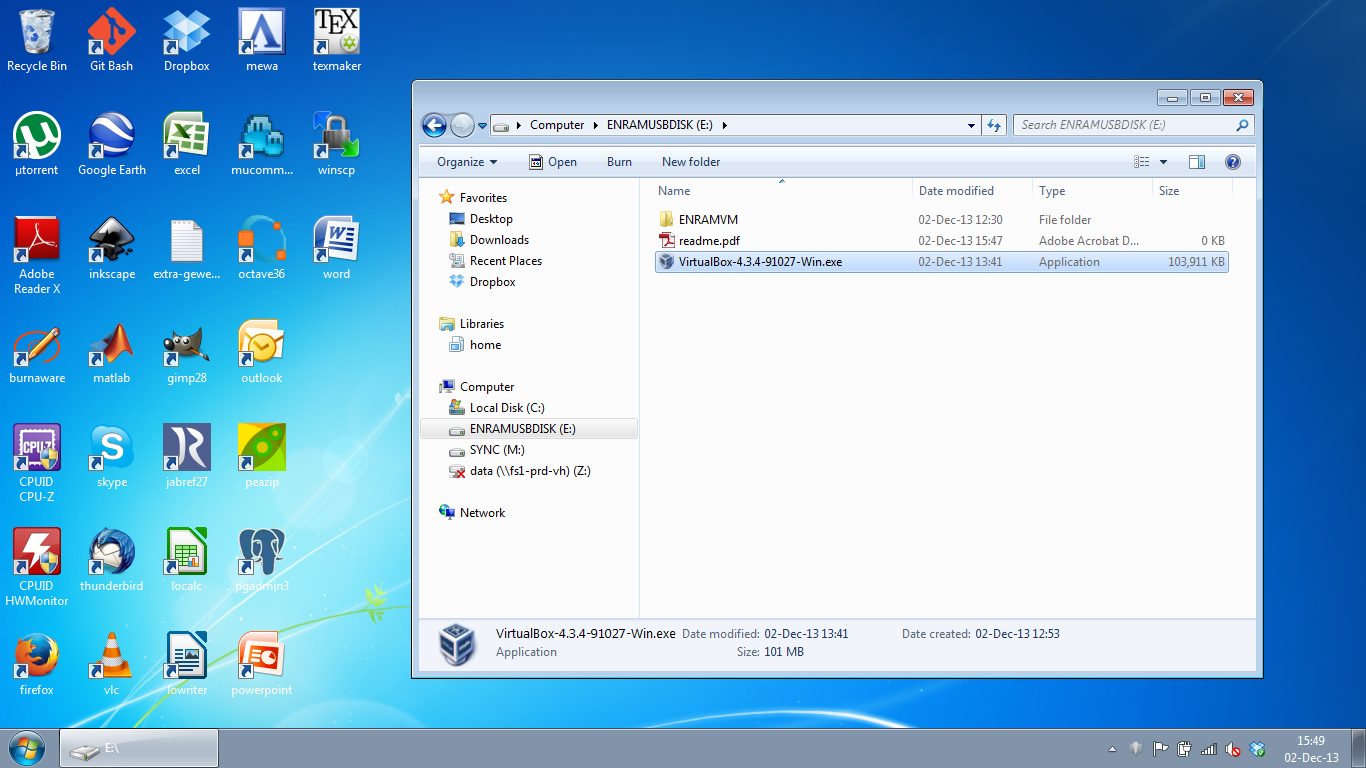
\includegraphics[width=0.85\linewidth , keepaspectratio]{./../eps/screenshot-1.eps}
  \caption{}
  \label{fig:screenshot-1}
\end{figure}


Double-click on the VirtualBox installer file (`VirtualBox-4.3.4-91027-Win.exe') to start the setup wizard. A menu will show up (Figure~\ref{fig:screenshot-2}). Click on the button labeled `Run'.

\begin{figure}[ht]
  \centering
    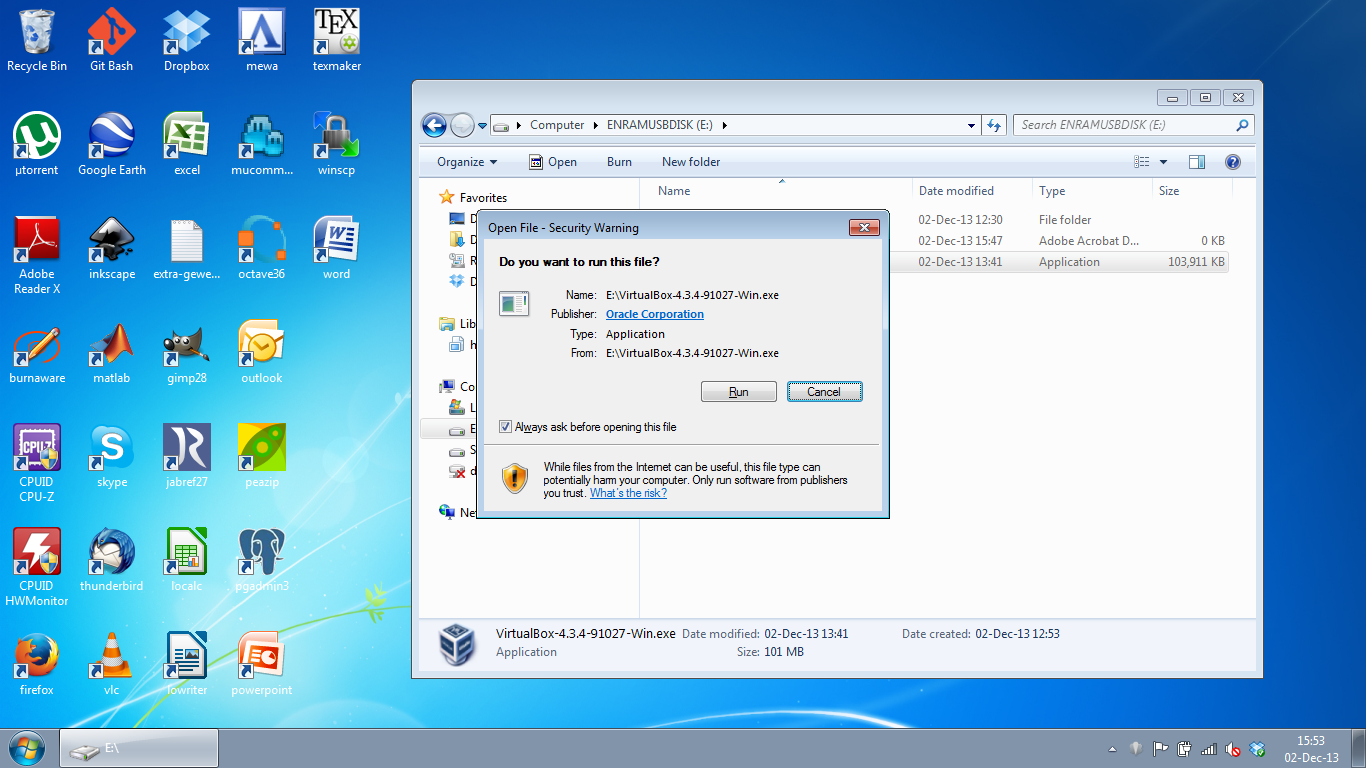
\includegraphics[width=0.80\linewidth , keepaspectratio]{./../eps/screenshot-2.eps}
  \caption{}
  \label{fig:screenshot-2}
\end{figure}
\clearpage


The setup wizard program should now start. On the first page of the setup wizard (Figure~\ref{fig:screenshot-3}), click the button labeled `Next'.

\begin{figure}[ht]
  \centering
    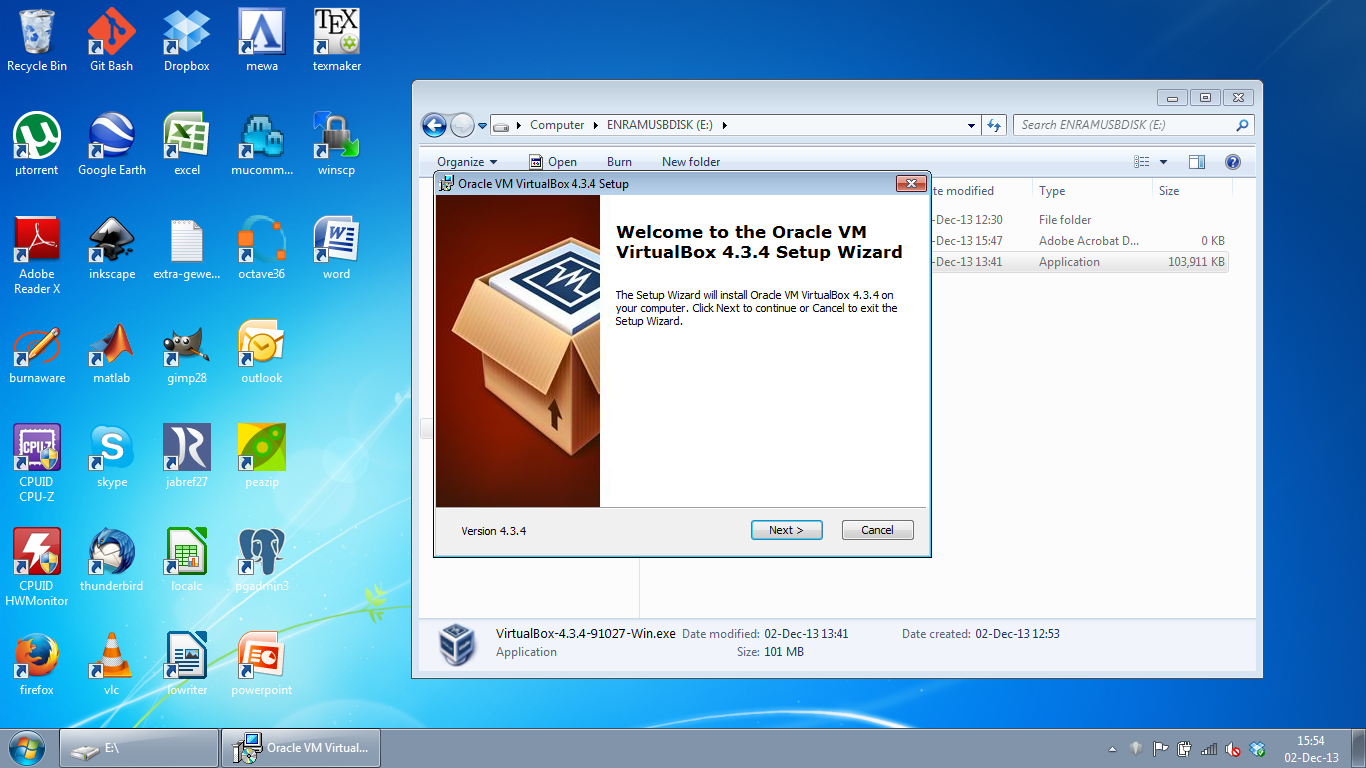
\includegraphics[width=0.80\linewidth , keepaspectratio]{./../eps/screenshot-3.eps}
  \caption{}
  \label{fig:screenshot-3}
\end{figure}


On the next page of the setup wizard (Figure~\ref{fig:screenshot-4}), click the button labeled `Next'.

\begin{figure}[ht]
  \centering
    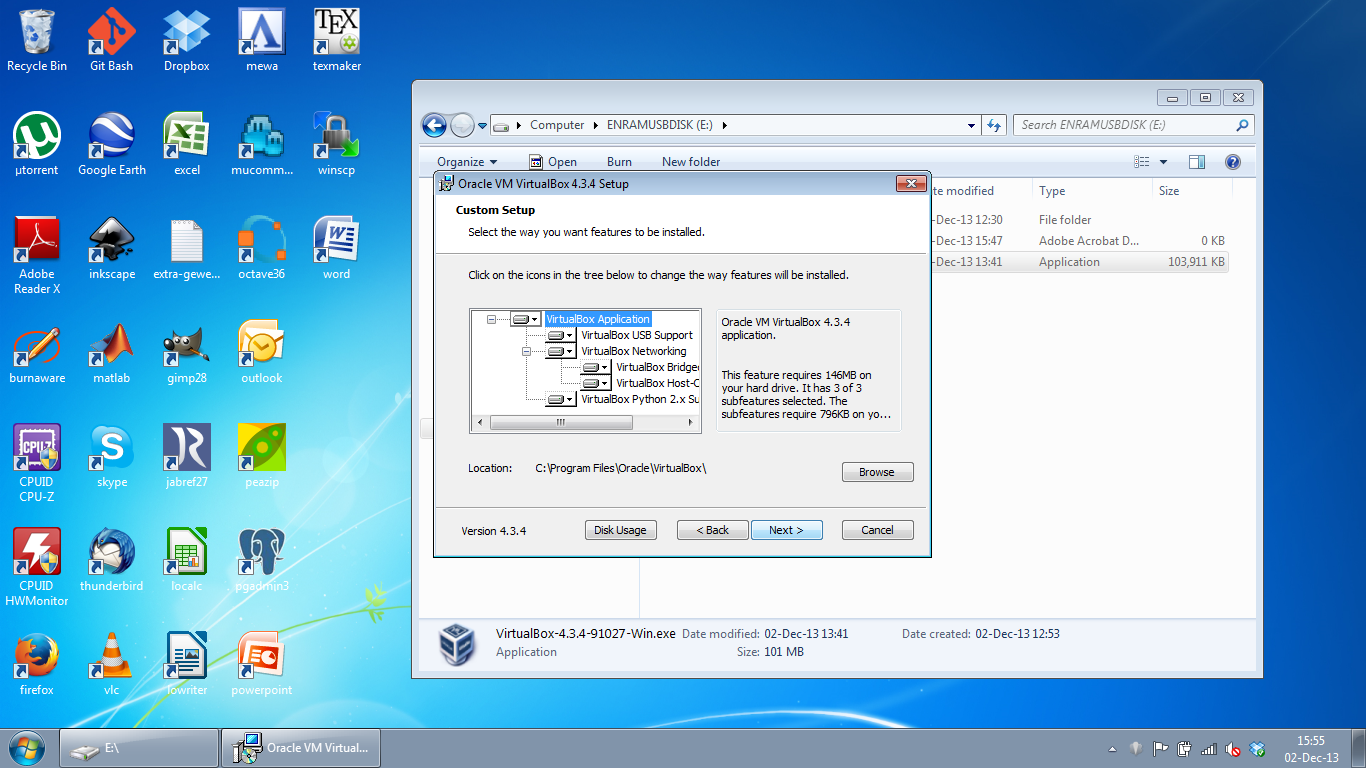
\includegraphics[width=0.80\linewidth , keepaspectratio]{./../eps/screenshot-4.eps}
  \caption{}
  \label{fig:screenshot-4}
\end{figure}
\clearpage

On the next page of the setup wizard (Figure~\ref{fig:screenshot-5}), check the items as you like. Then click the button labeled `Next'.

\begin{figure}[ht]
  \centering
    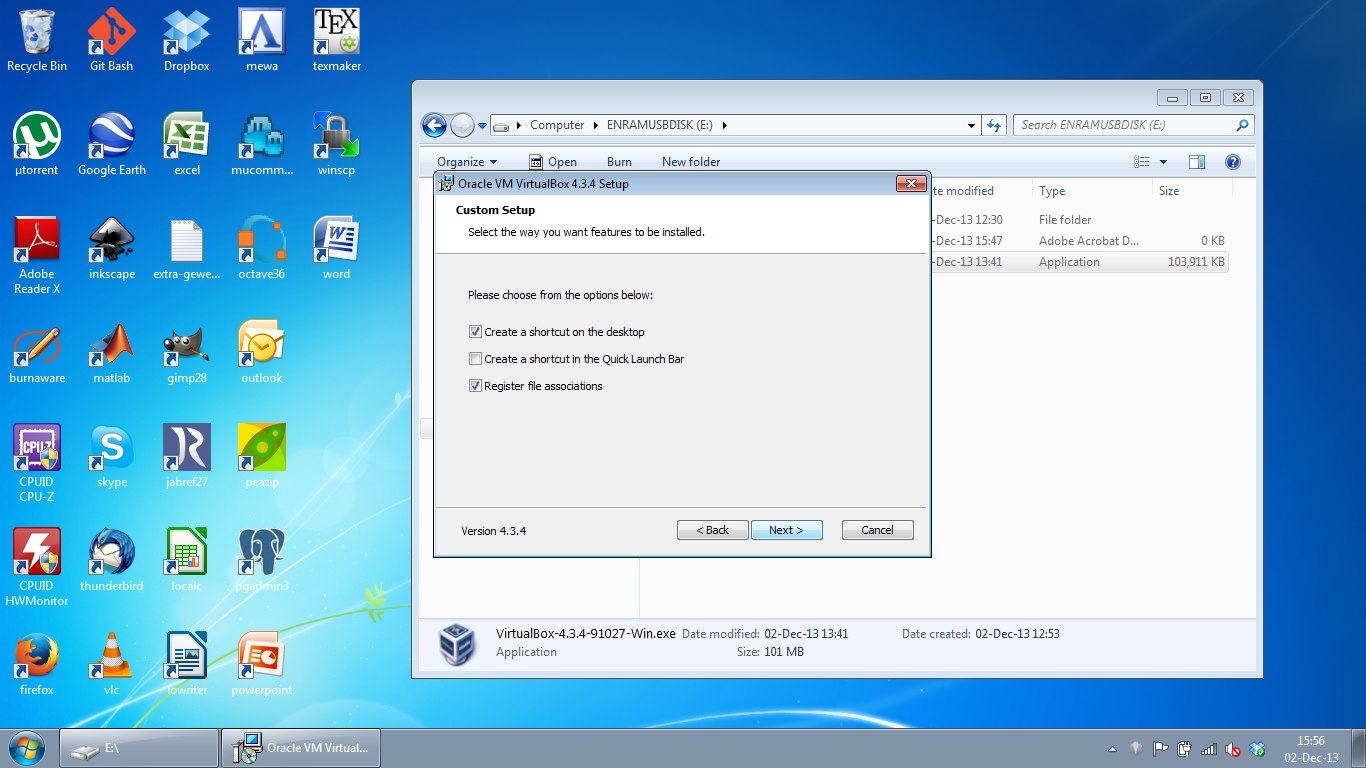
\includegraphics[width=0.80\linewidth , keepaspectratio]{./../eps/screenshot-5.eps}
  \caption{}
  \label{fig:screenshot-5}
\end{figure}


Make sure you are not currently doing something that requires network access (like downloading a big file). Then, on the next page of the setup wizard (Figure~\ref{fig:screenshot-6}), click the button labeled `Yes'.

\begin{figure}[ht]
  \centering
    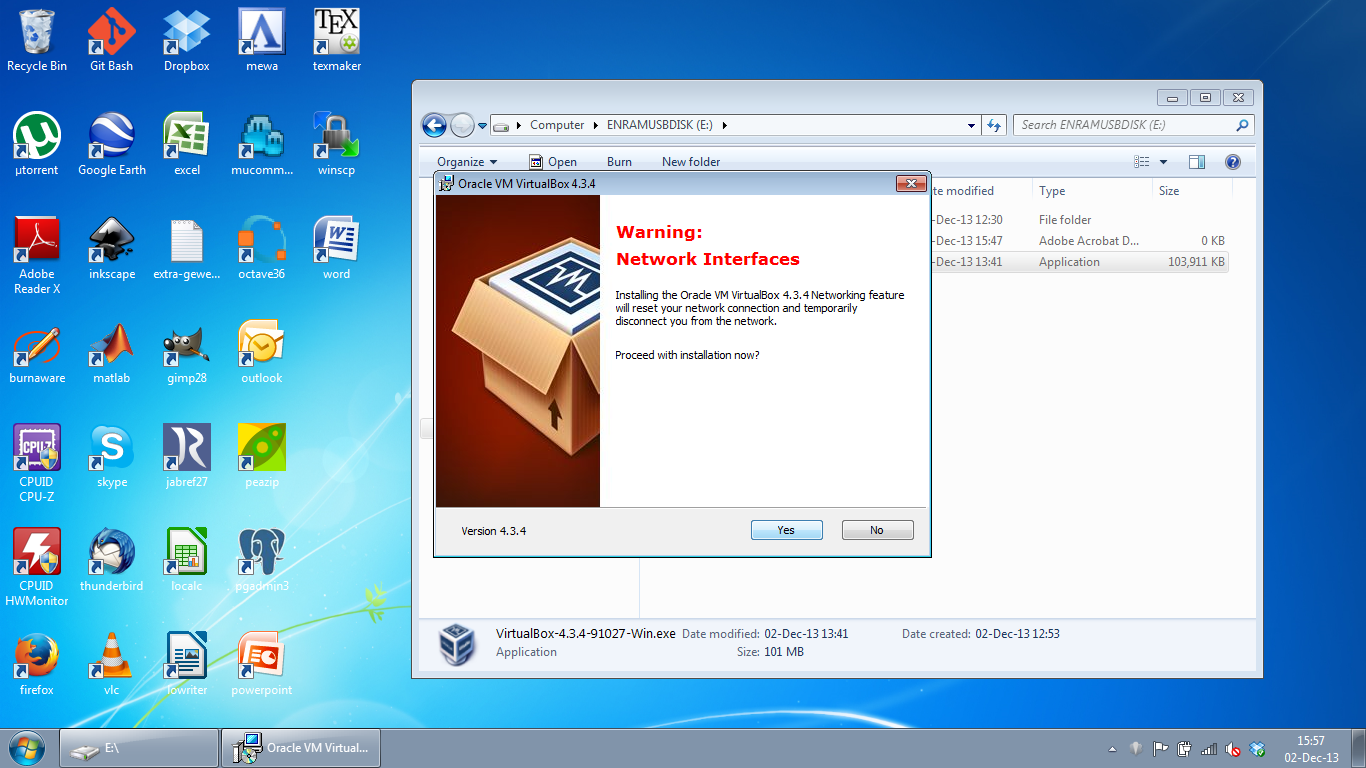
\includegraphics[width=0.80\linewidth , keepaspectratio]{./../eps/screenshot-6.eps}
  \caption{}
  \label{fig:screenshot-6}
\end{figure}
\clearpage

On the next page of the setup wizard, click the button labeled `Install'.

\begin{figure}[ht]
  \centering
    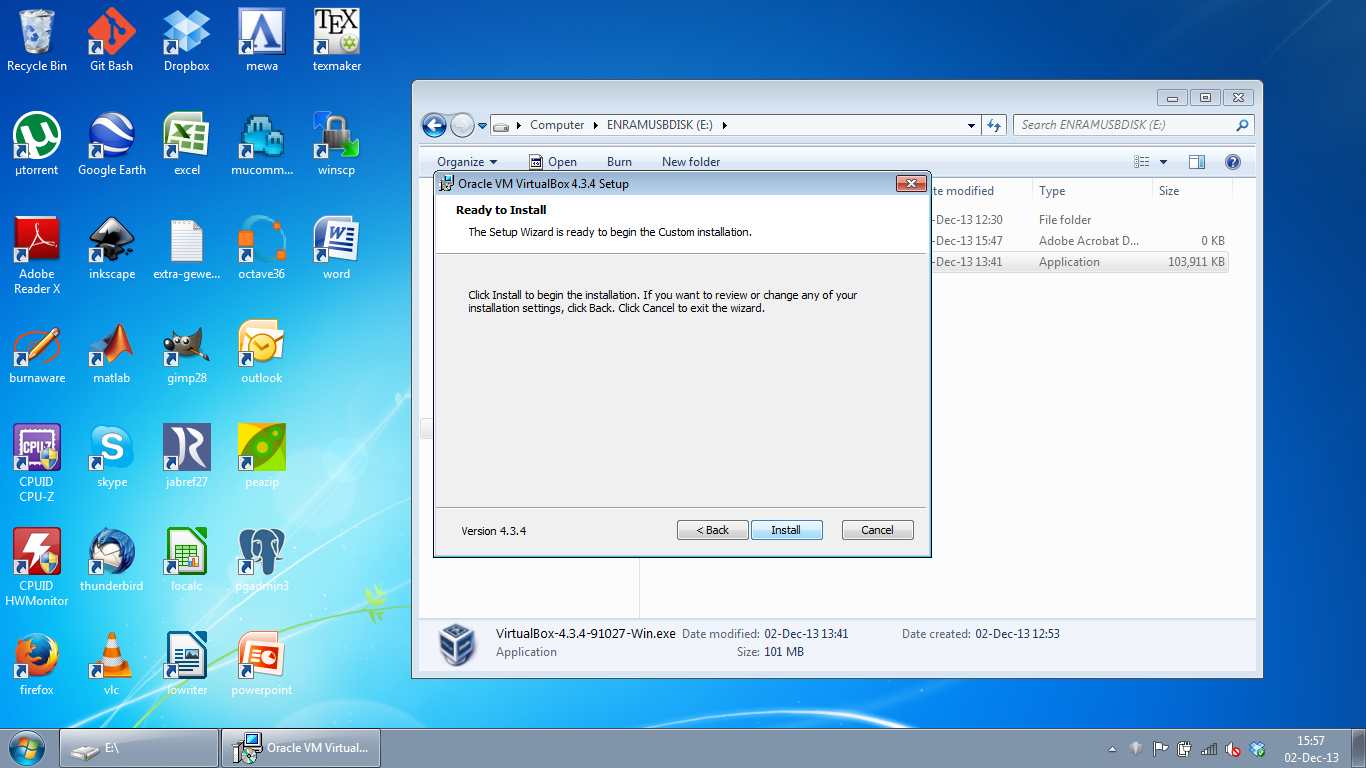
\includegraphics[width=0.80\linewidth , keepaspectratio]{./../eps/screenshot-7.eps}
  \caption{}
  \label{fig:screenshot-7}
\end{figure}



Allright! Looks like you just installed VirtualBox. Leave the checkbox checked (Figure~\ref{fig:screenshot-9}) and click on the button labeled `Finish'.
\begin{figure}[ht]
  \centering
    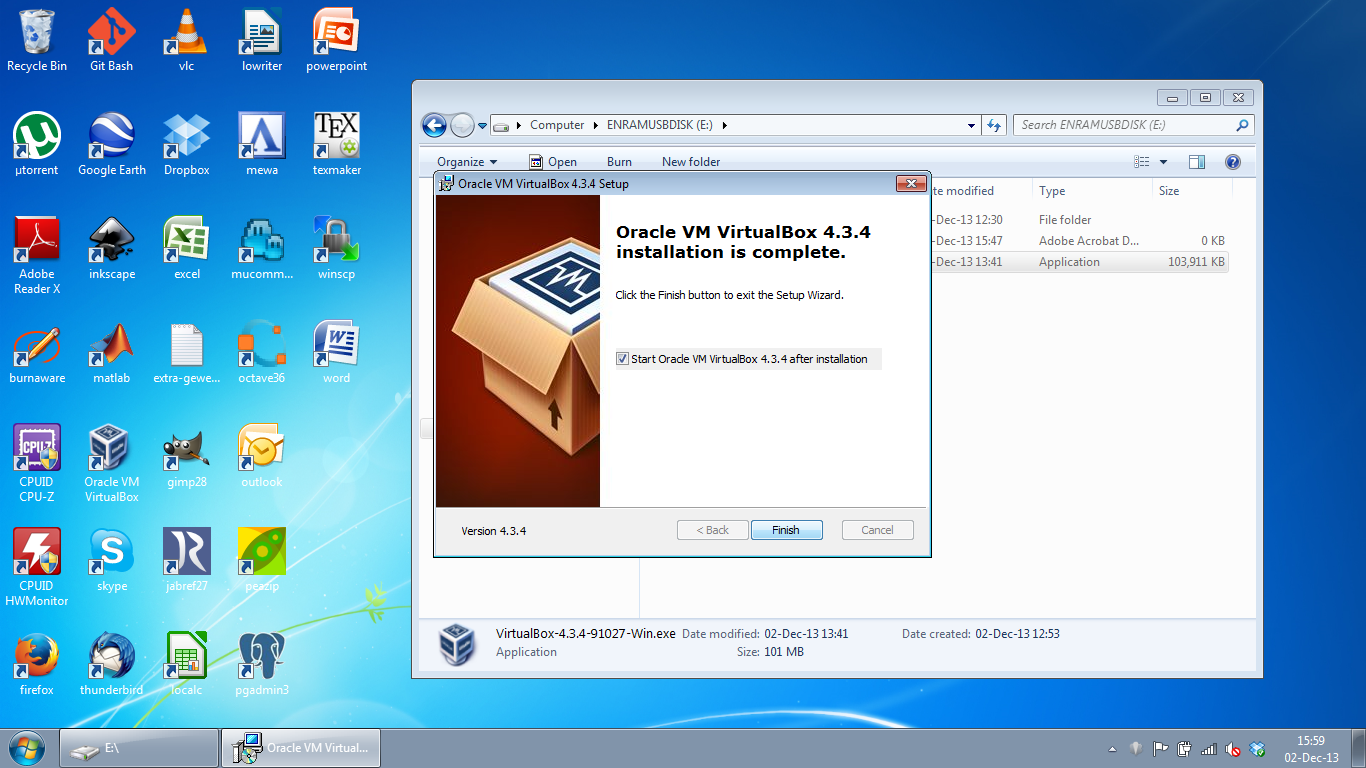
\includegraphics[width=0.80\linewidth , keepaspectratio]{./../eps/screenshot-9.eps}
  \caption{}
  \label{fig:screenshot-9}
\end{figure}
\clearpage


\section{Creating a virtual machine and running it}
\label{sec:creating-virtual-machine}

Before we can access all the goodies that are on the virtual disk, we need to create a so-called \textit{virtual machine}. Start the VirtualBox program if it has not already started. Since this probably is the first time you started VirtualBox, the program will show a welcome message (Figure~\ref{fig:screenshot-10}). Click on light blue icon in the top left corner labeled `New'.

\begin{figure}[ht]
  \centering
    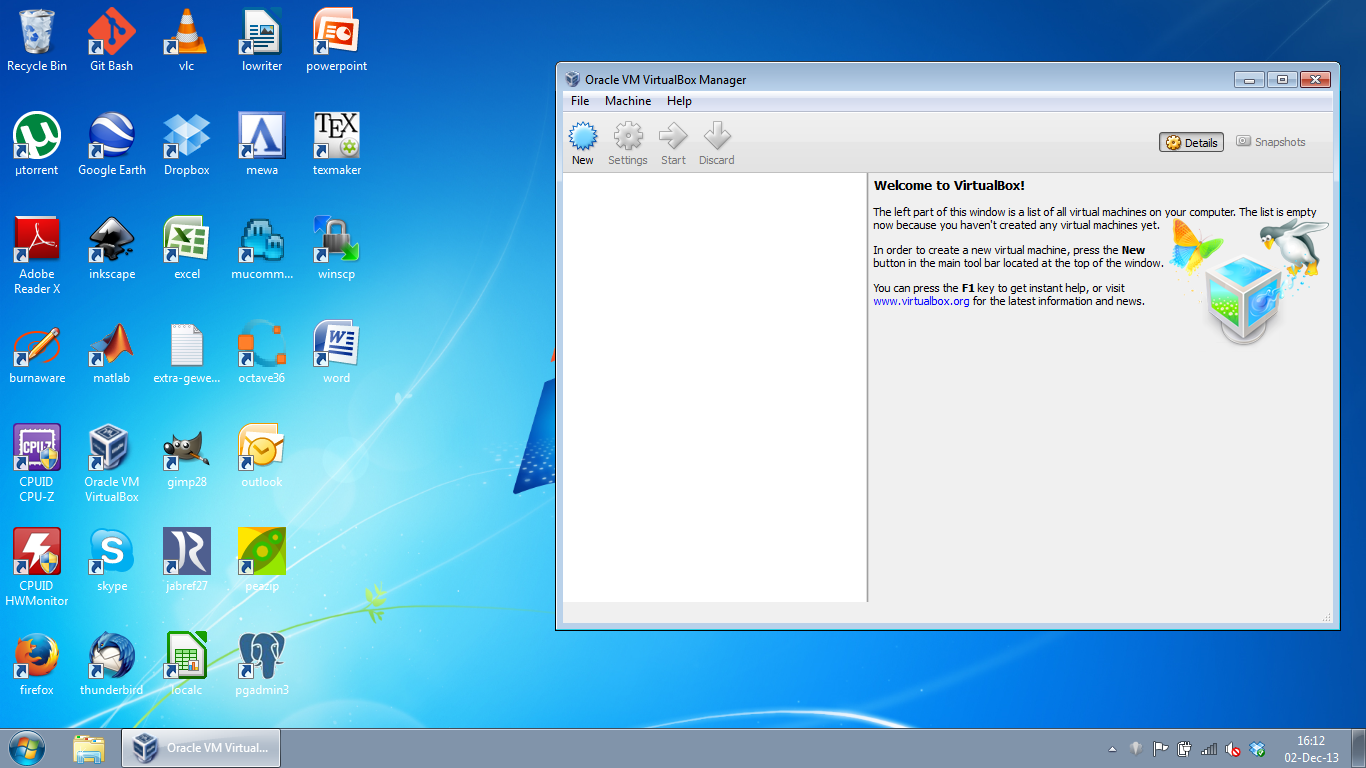
\includegraphics[width=0.80\linewidth , keepaspectratio]{./../eps/screenshot-10.eps}
  \caption{}
  \label{fig:screenshot-10}
\end{figure}


In this window (Figure~\ref{fig:screenshot-11}), specify `ENRAMVM' as the name of the virtual machine.

Use the drop-down menus to choose the type of operating system (`Linux') and the version (`Ubuntu 64-bit').

Click the button labeled `Next'.


\begin{figure}[ht]
  \centering
    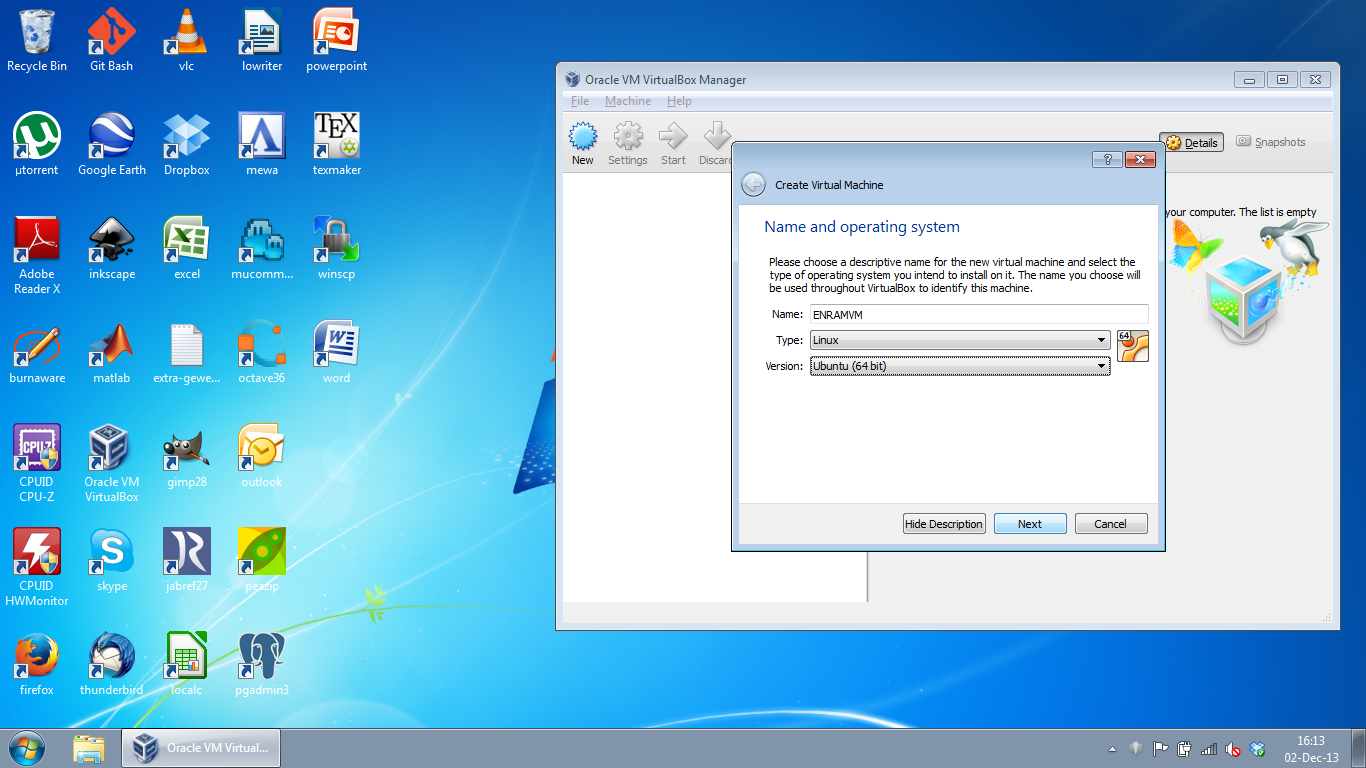
\includegraphics[width=0.80\linewidth , keepaspectratio]{./../eps/screenshot-11.eps}
  \caption{}
  \label{fig:screenshot-11}
\end{figure}
\clearpage

In this window, you need to specify the amount of virtual memory that your virtual machine will have. Set it to 4096 MB (Figure~\ref{fig:screenshot-12}).

Click the button labeled `Next'.

\begin{figure}[ht]
  \centering
    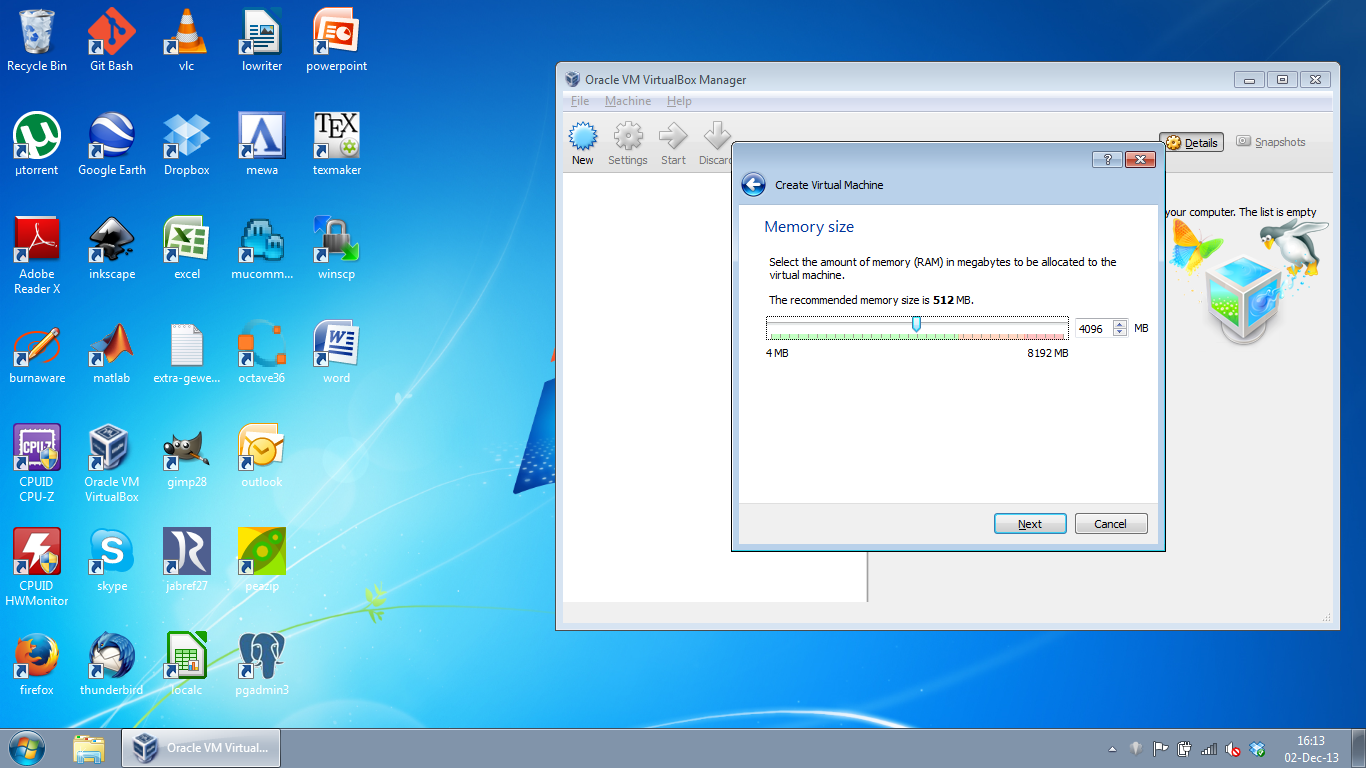
\includegraphics[width=0.80\linewidth , keepaspectratio]{./../eps/screenshot-12.eps}
  \caption{}
  \label{fig:screenshot-12}
\end{figure}


In this window, make sure to choose the last option `Use an existing virtual hard drive file'. Use the little folder icon to the right of the drop-down list to select the virtual hard drive file `ENRAMVM Clone-disk1.vdi' that is located in folder `ENRAMVM' on ENRAMUSBDISK.

Then, click the button labeled `Create'.

\begin{figure}[ht]
  \centering
    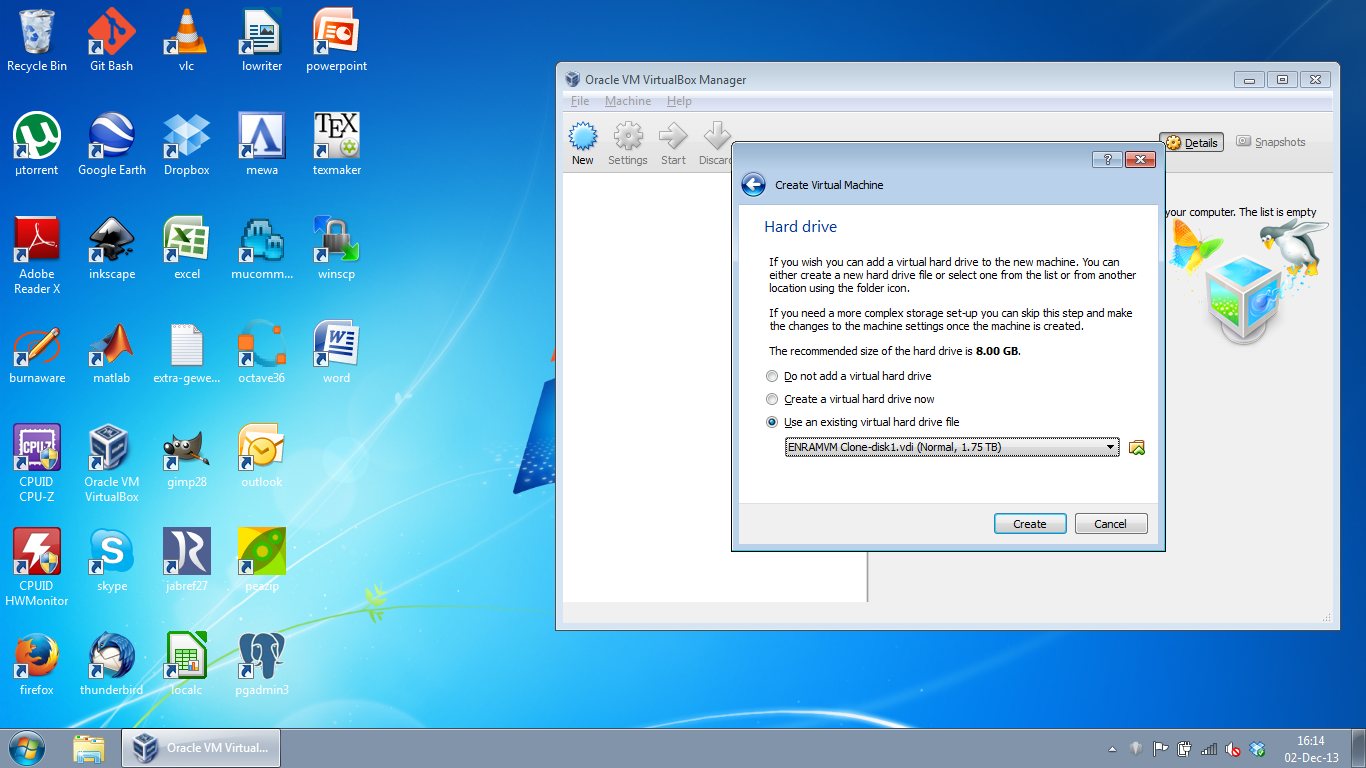
\includegraphics[width=0.80\linewidth , keepaspectratio]{./../eps/screenshot-13.eps}
  \caption{}
  \label{fig:screenshot-13}
\end{figure}
\clearpage

Sweet! We have a virtual machine (`ENRAMVM'; Figure~\ref{fig:screenshot-14}). Boot up the virtual machine by clicking the icon with the green arrow labeled `Start'.

\begin{figure}[ht]
  \centering
    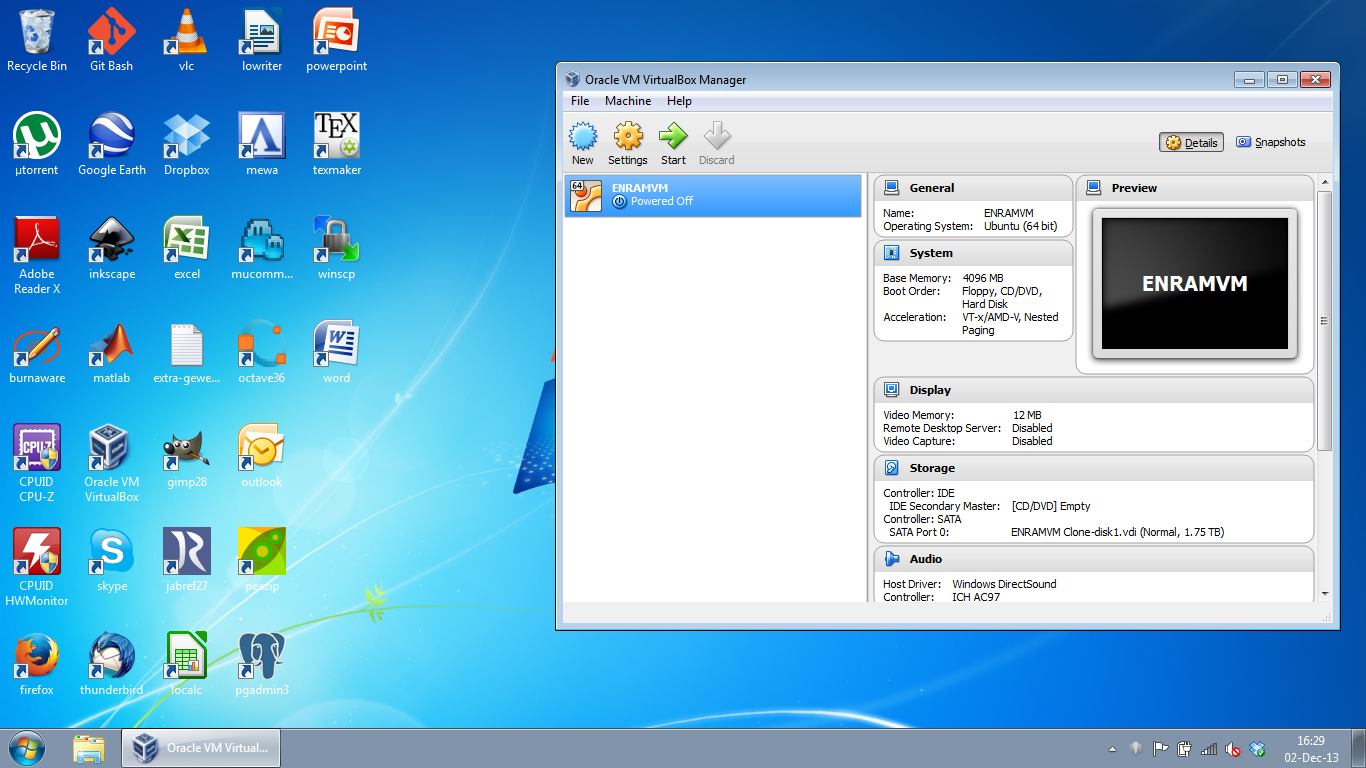
\includegraphics[width=0.80\linewidth , keepaspectratio]{./../eps/screenshot-14.eps}
  \caption{}
  \label{fig:screenshot-14}
\end{figure}


A new Window will pop up (Figure~\ref{fig:screenshot-15}), which initially is just black, but after a couple of seconds, stuff will appear. There will likely also be two warning messages, but you can ignore these by clicking on the little blue icon in the top right corner of the ENRAMVM window.


\begin{figure}[ht]
  \centering
    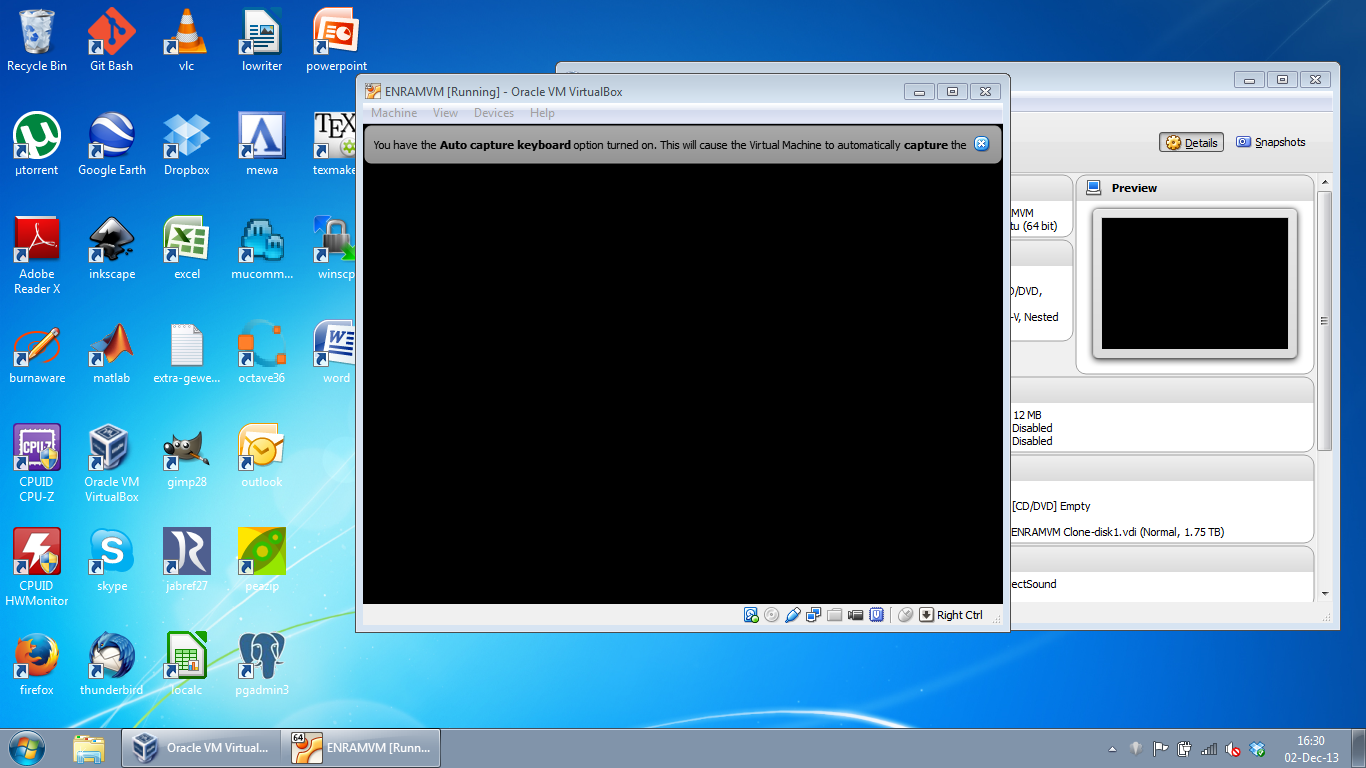
\includegraphics[width=0.80\linewidth , keepaspectratio]{./../eps/screenshot-15.eps}
  \caption{}
  \label{fig:screenshot-15}
\end{figure}
\clearpage

After a couple more seconds, your newly created ENRAMVM machine will have finished booting and will be ready for you to use. It will show you a blue desktop with a few icons on it (Figure~\ref{fig:screenshot-16}).

\begin{figure}[ht]
  \centering
    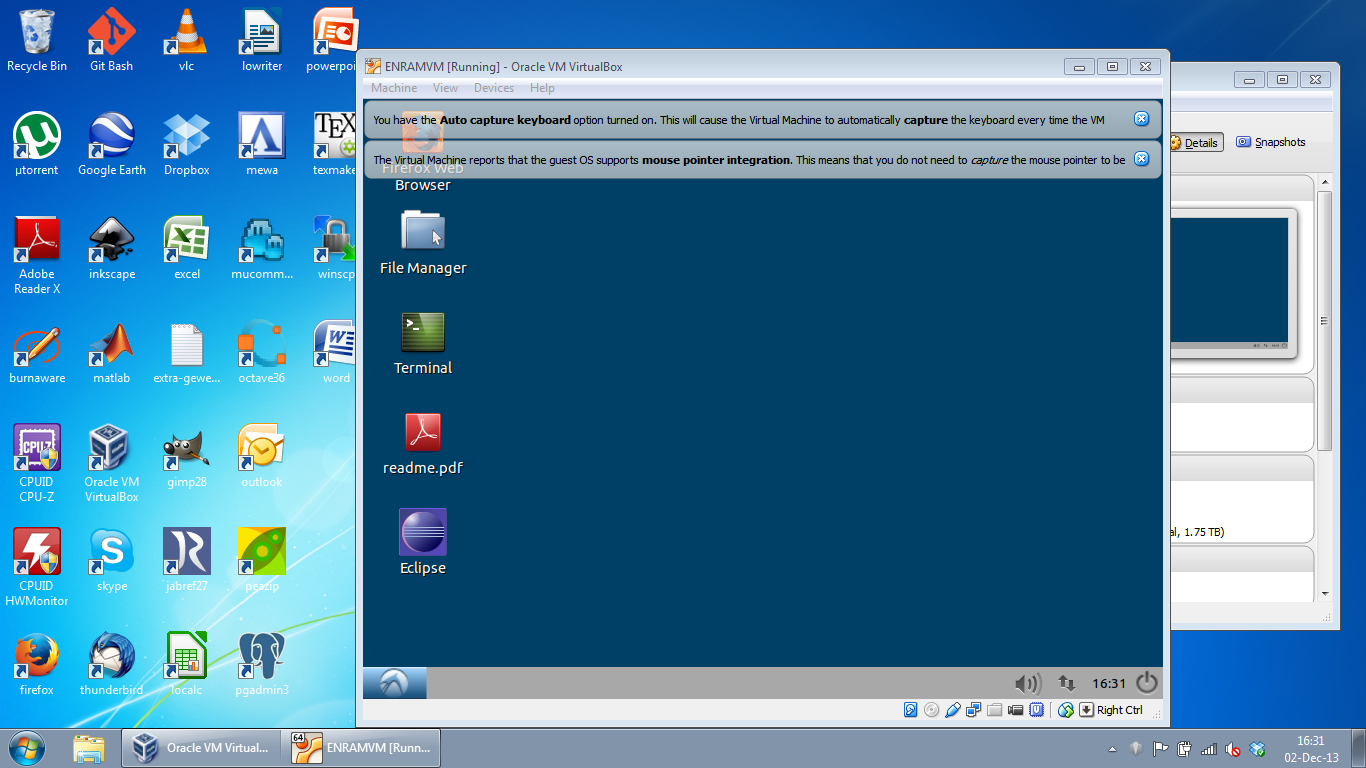
\includegraphics[width=0.80\linewidth , keepaspectratio]{./../eps/screenshot-16.eps}
  \caption{}
  \label{fig:screenshot-16}
\end{figure}


Before we do anything else, let's first maximize the virtual screen. You can do this by clicking on the menu item `View' and then selecting `Switch to Fullscreen' (Figure~\ref{fig:screenshot-17}).

\begin{figure}[ht]
  \centering
    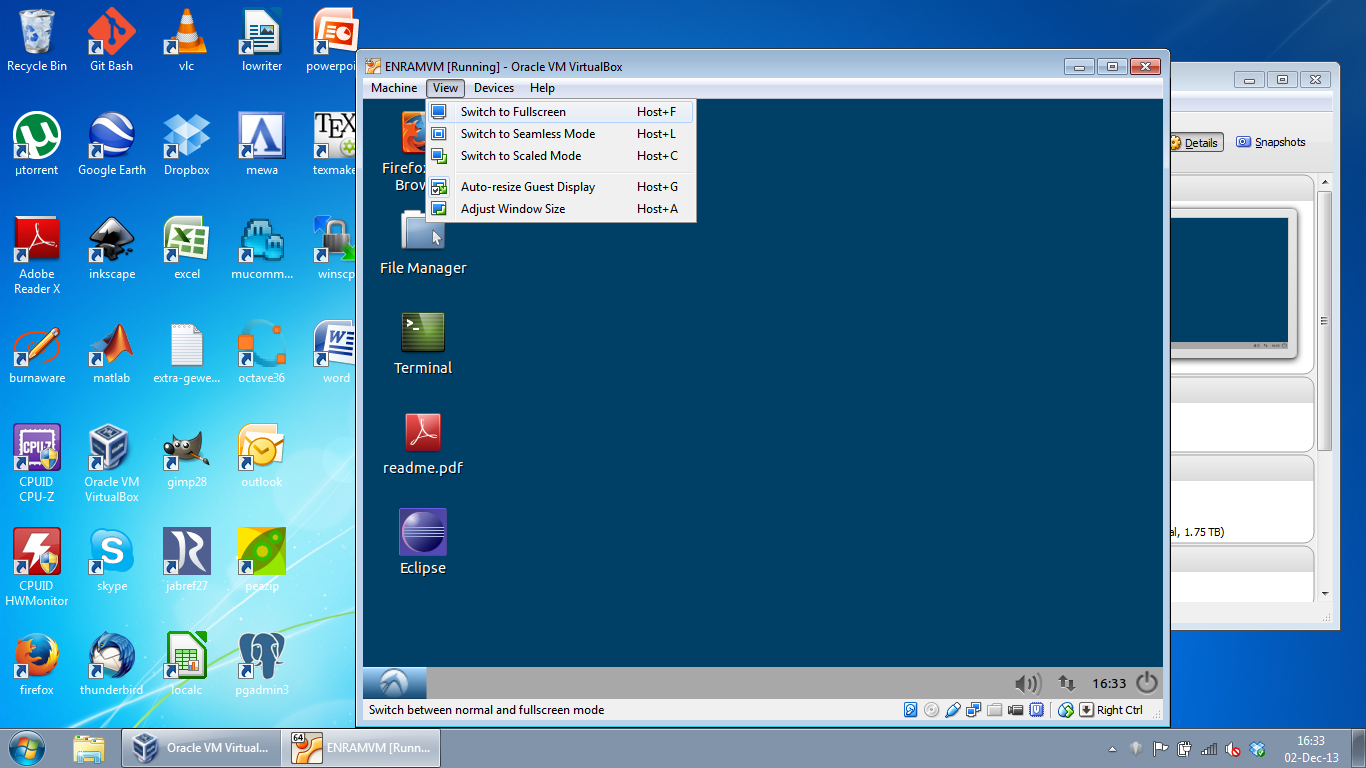
\includegraphics[width=0.80\linewidth , keepaspectratio]{./../eps/screenshot-17.eps}
  \caption{}
  \label{fig:screenshot-17}
\end{figure}
\clearpage


Note that you can toggle between fullscreen and windowed mode by simultaneously pressing the letter F button and the Ctrl button on the right hand side of your keyboard (Figure~\ref{fig:screenshot-18}).

Click the `Switch' button to switch to Fullscreen mode.

\begin{figure}[ht]
  \centering
    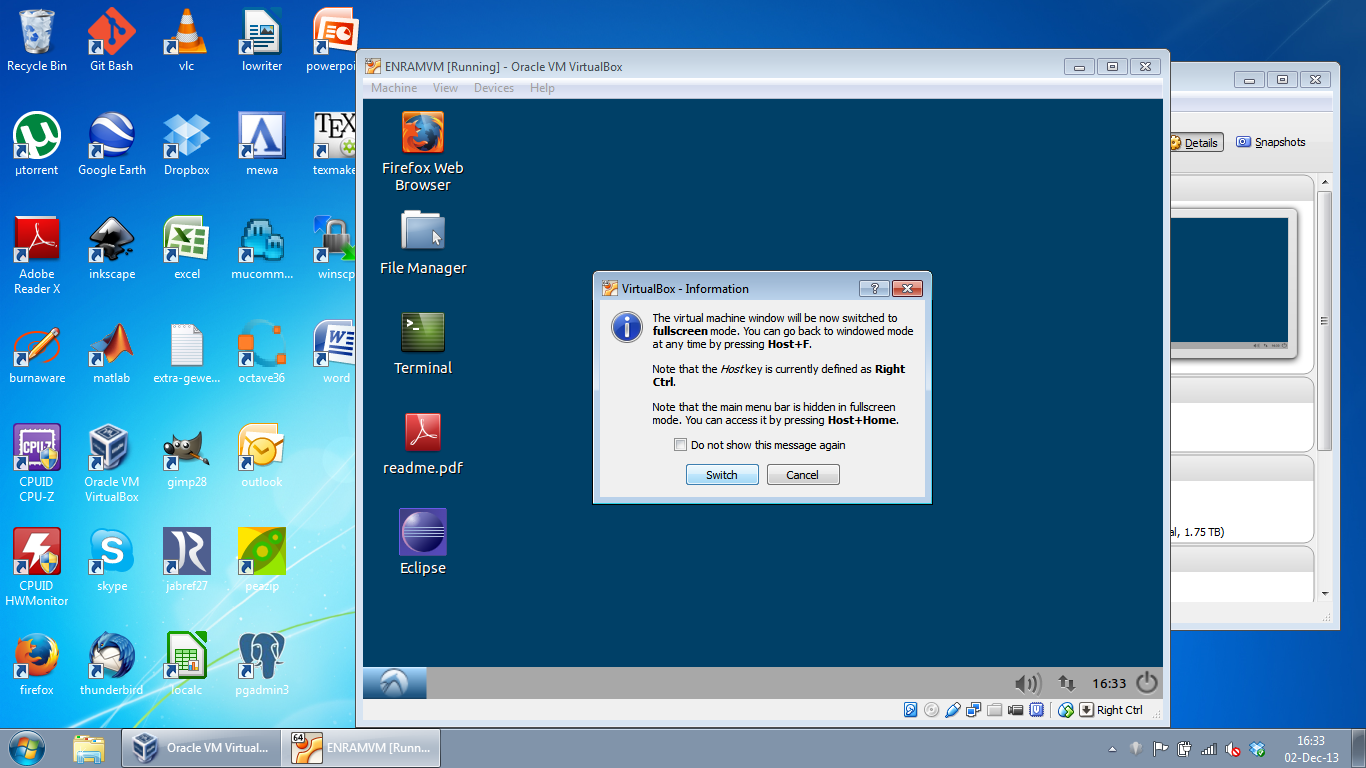
\includegraphics[width=0.80\linewidth , keepaspectratio]{./../eps/screenshot-18.eps}
  \caption{}
  \label{fig:screenshot-18}
\end{figure}

You should now see the virtual machine's desktop fullscreen (Figure~\ref{fig:screenshot-19}).

\begin{figure}[ht]
  \centering
    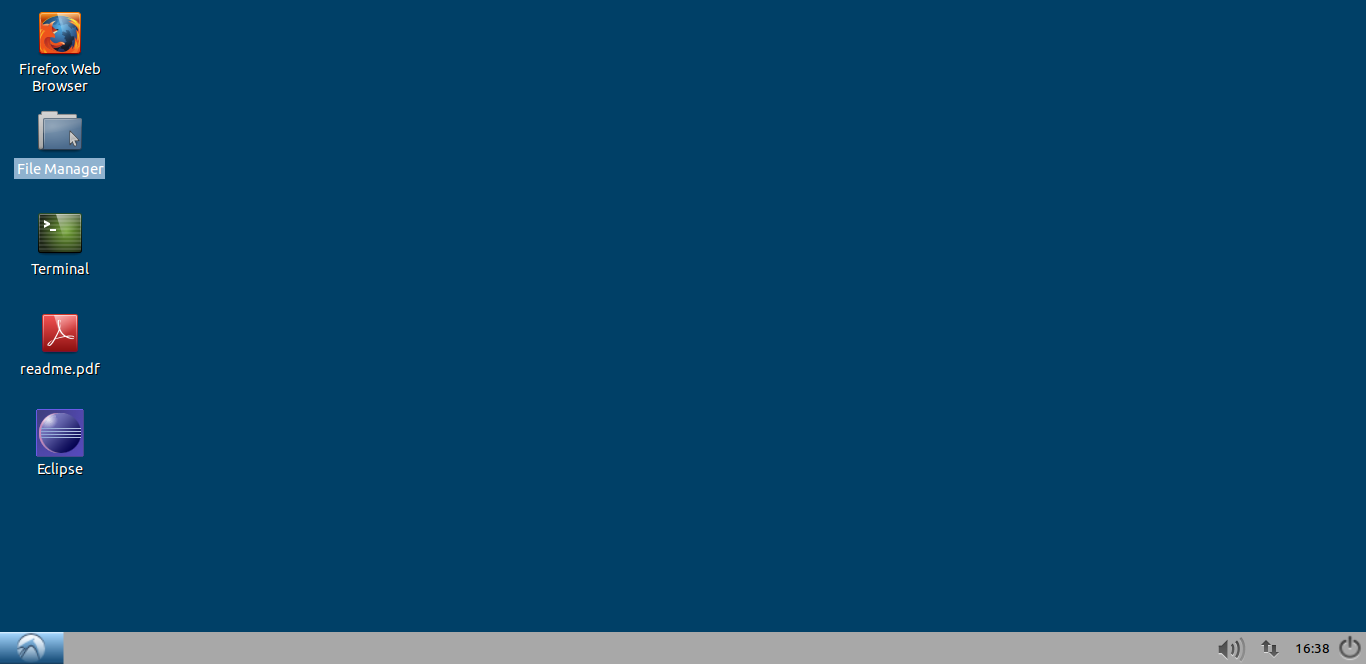
\includegraphics[width=0.80\linewidth , keepaspectratio]{./../eps/screenshot-19.eps}
  \caption{}
  \label{fig:screenshot-19}
\end{figure}
\clearpage

%\begin{figure}[ht]
  %\centering
    %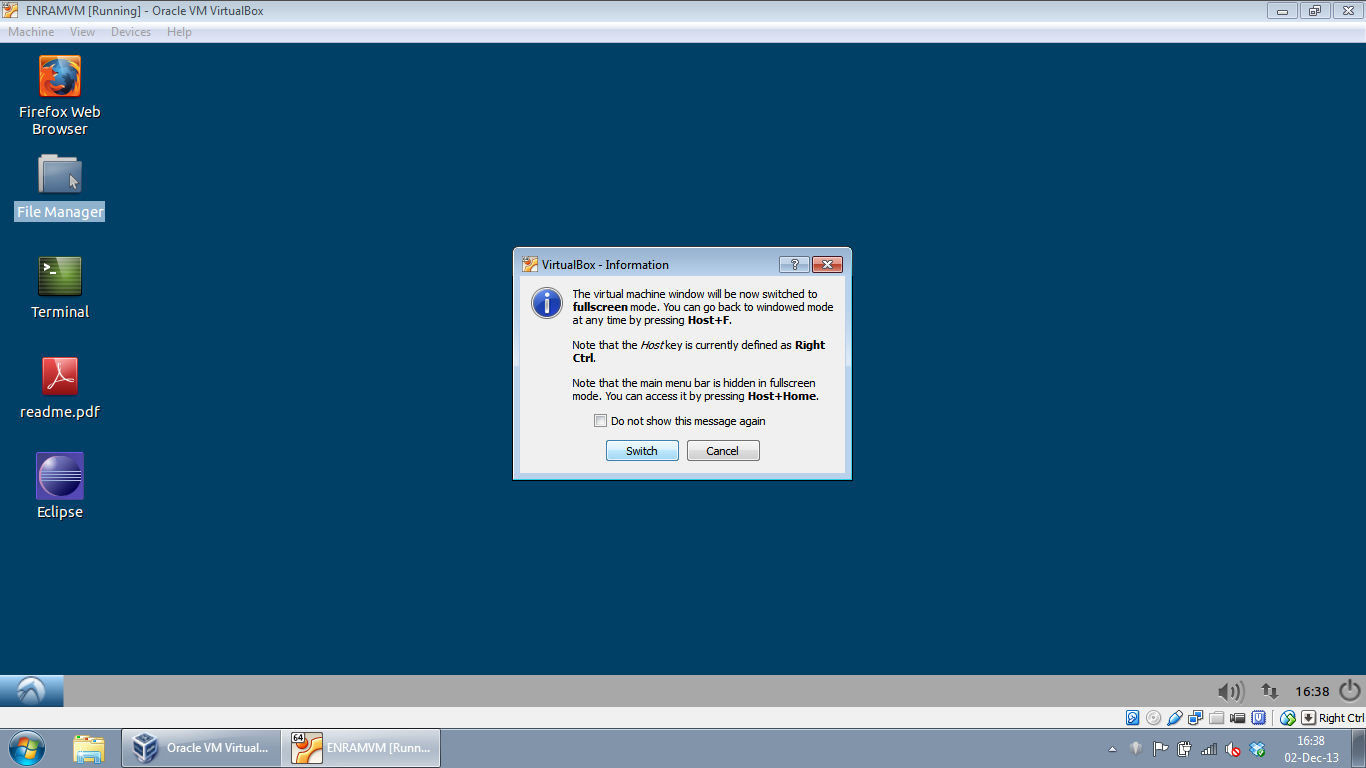
\includegraphics[width=0.80\linewidth , keepaspectratio]{./../eps/screenshot-20.eps}
  %\caption{screenshot 20}
  %\label{fig:screenshot-20}
%\end{figure}

The next chapter explains how to use the ENRAM software and data, but at some point you'll want to power down the virtual machine, so let's look at that first.

Click on the blue icon in the taskbar in the lower left corner of the screen, and choose `Logout' (Figure~\ref{fig:screenshot-21}).

\begin{figure}[ht]
  \centering
    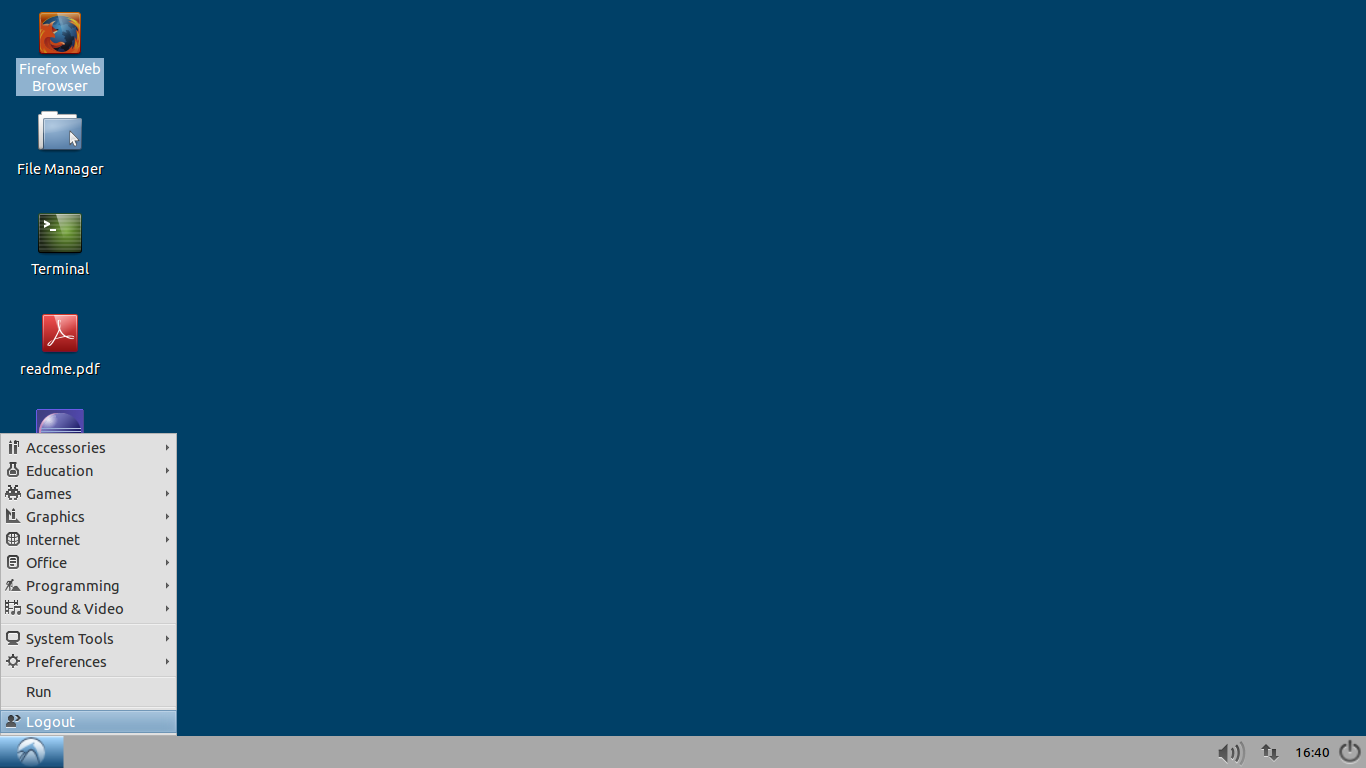
\includegraphics[width=0.80\linewidth , keepaspectratio]{./../eps/screenshot-21.eps}
  \caption{}
  \label{fig:screenshot-21}
\end{figure}
\clearpage

In this menu, choose `Shutdown' to power down the virtual machine (Figure~\ref{fig:screenshot-22}). After a few seconds, you will be back at you Windows desktop (Figure~\ref{fig:screenshot-23}).

\begin{figure}[ht]
  \centering
    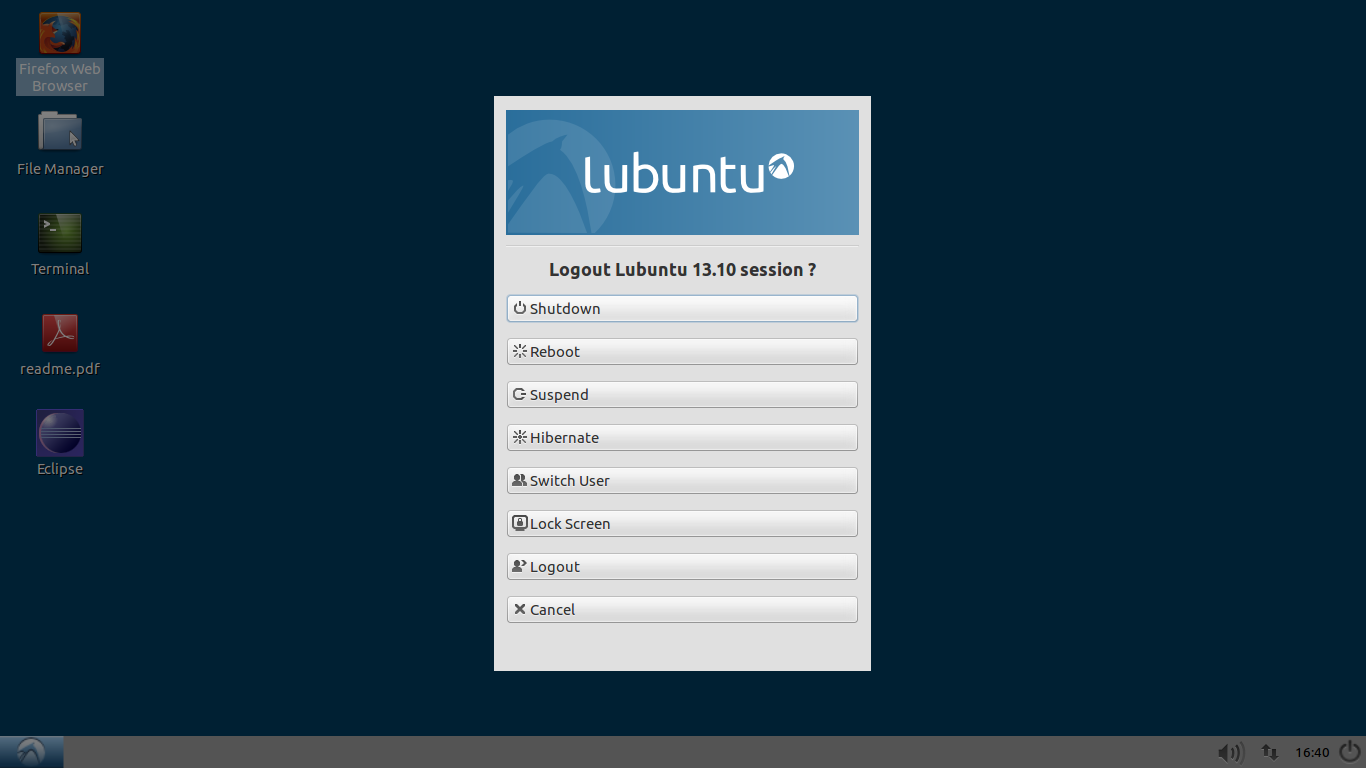
\includegraphics[width=0.80\linewidth , keepaspectratio]{./../eps/screenshot-22.eps}
  \caption{}
  \label{fig:screenshot-22}
\end{figure}

\begin{figure}[hb]
  \centering
    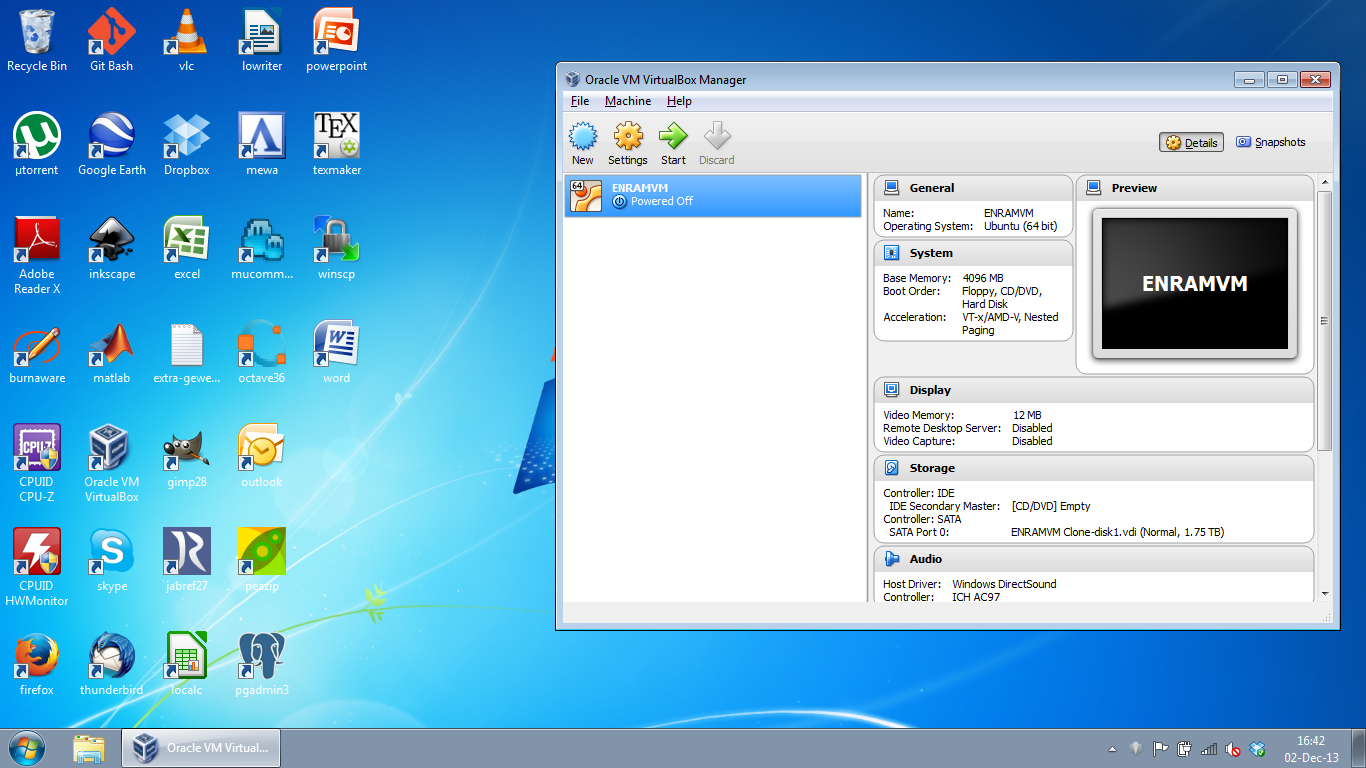
\includegraphics[width=0.80\linewidth , keepaspectratio]{./../eps/screenshot-23.eps}
  \caption{}
  \label{fig:screenshot-23}
\end{figure}




\chapter{Using the ENRAM software}
\label{ch:using-the-enram-software}


Make sure you have your virtual machine running (as in Figure~\ref{fig:screenshot-19}). 

Start the File Manager by clicking on the desktop icon labeled `File Manager'. In the file manager window, double-click on the directory called `enram' to inspect its contents.

Start a terminal by double-clicking the desktop icon labeled `Terminal'. This should bring up a terminal program (Figure~\ref{fig:screenshot-24}). In the terminal window, use the \texttt{cd} command to change directory into the `enram' directory. 

\begin{figure}[ht]
  \centering
    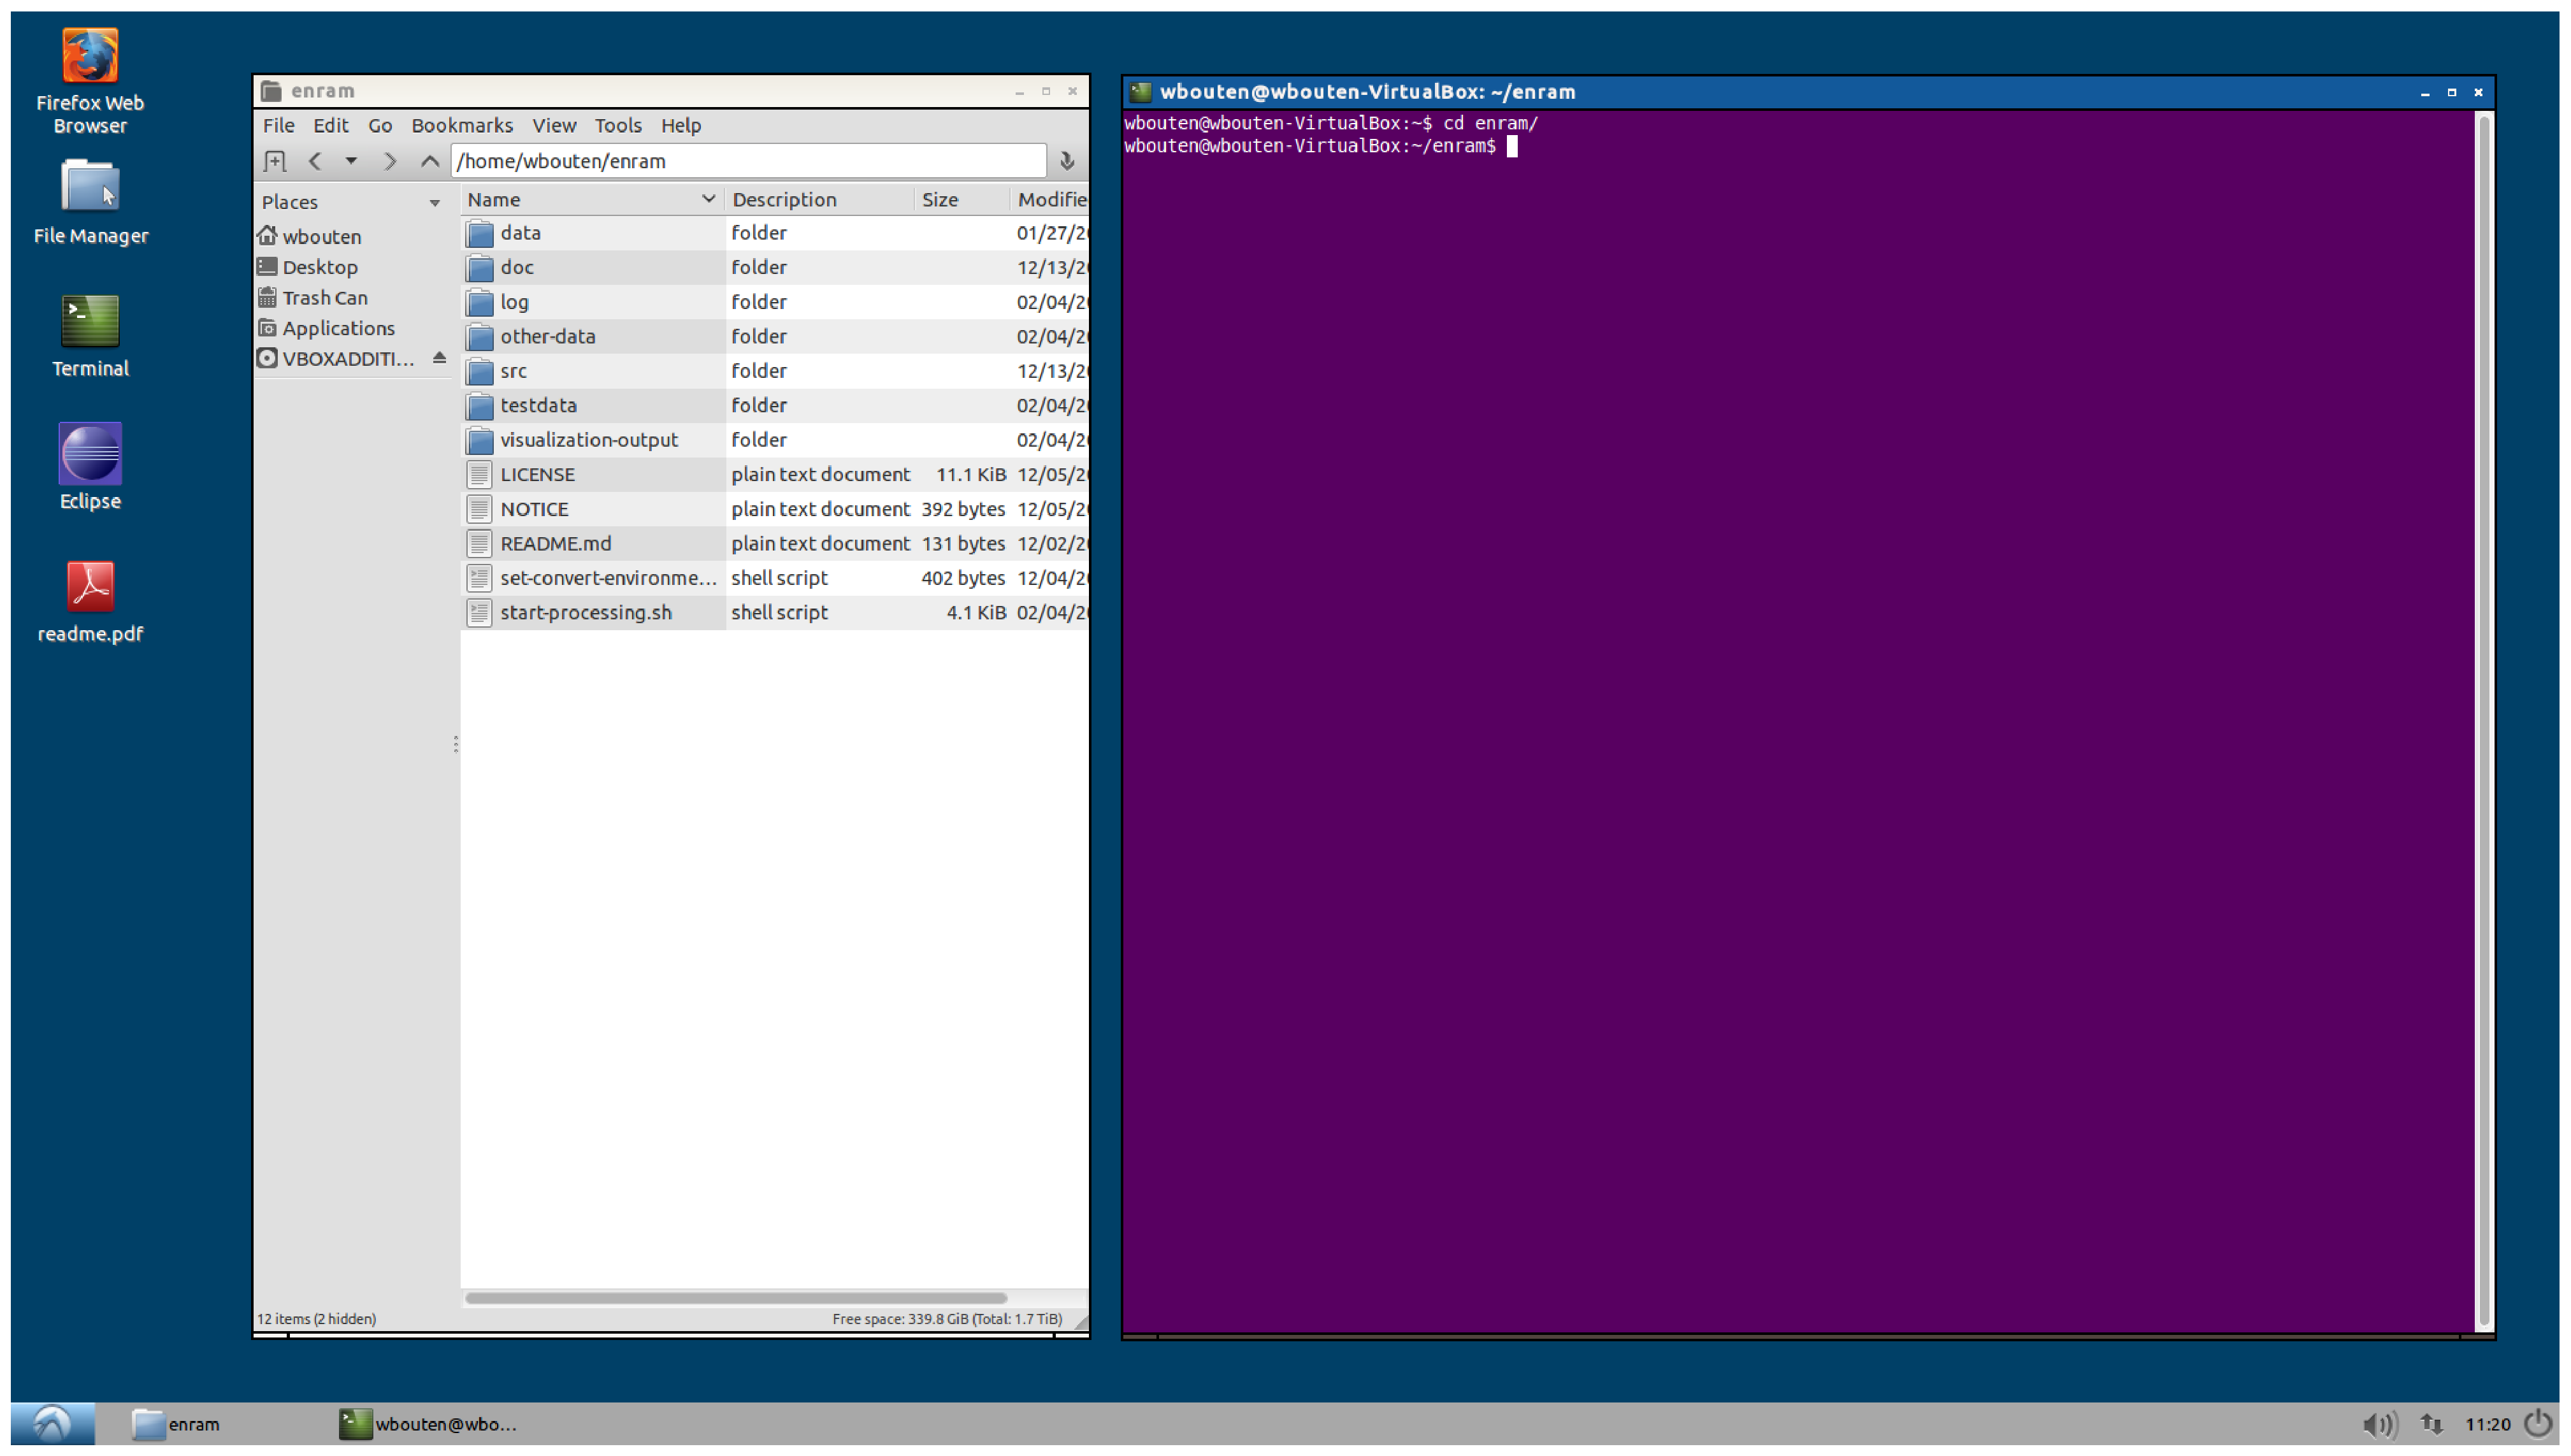
\includegraphics[width=0.85\linewidth , keepaspectratio]{./../eps/screenshot-24.eps}
  \caption{}
  \label{fig:screenshot-24}
\end{figure}


You can now start the ENRAM workflow as follows. Type:\\
\texttt{. ./start-processing.sh}

(But make sure to type it exactly as it is displayed here, including the leading dot).

The terminal will then first ask you whether you want an interactive session or you want to start processing in batch mode; then it will ask you to select either the test data set or the full data set (Figure~\ref{fig:screenshot-25}).

\begin{figure}[ht]
  \centering
    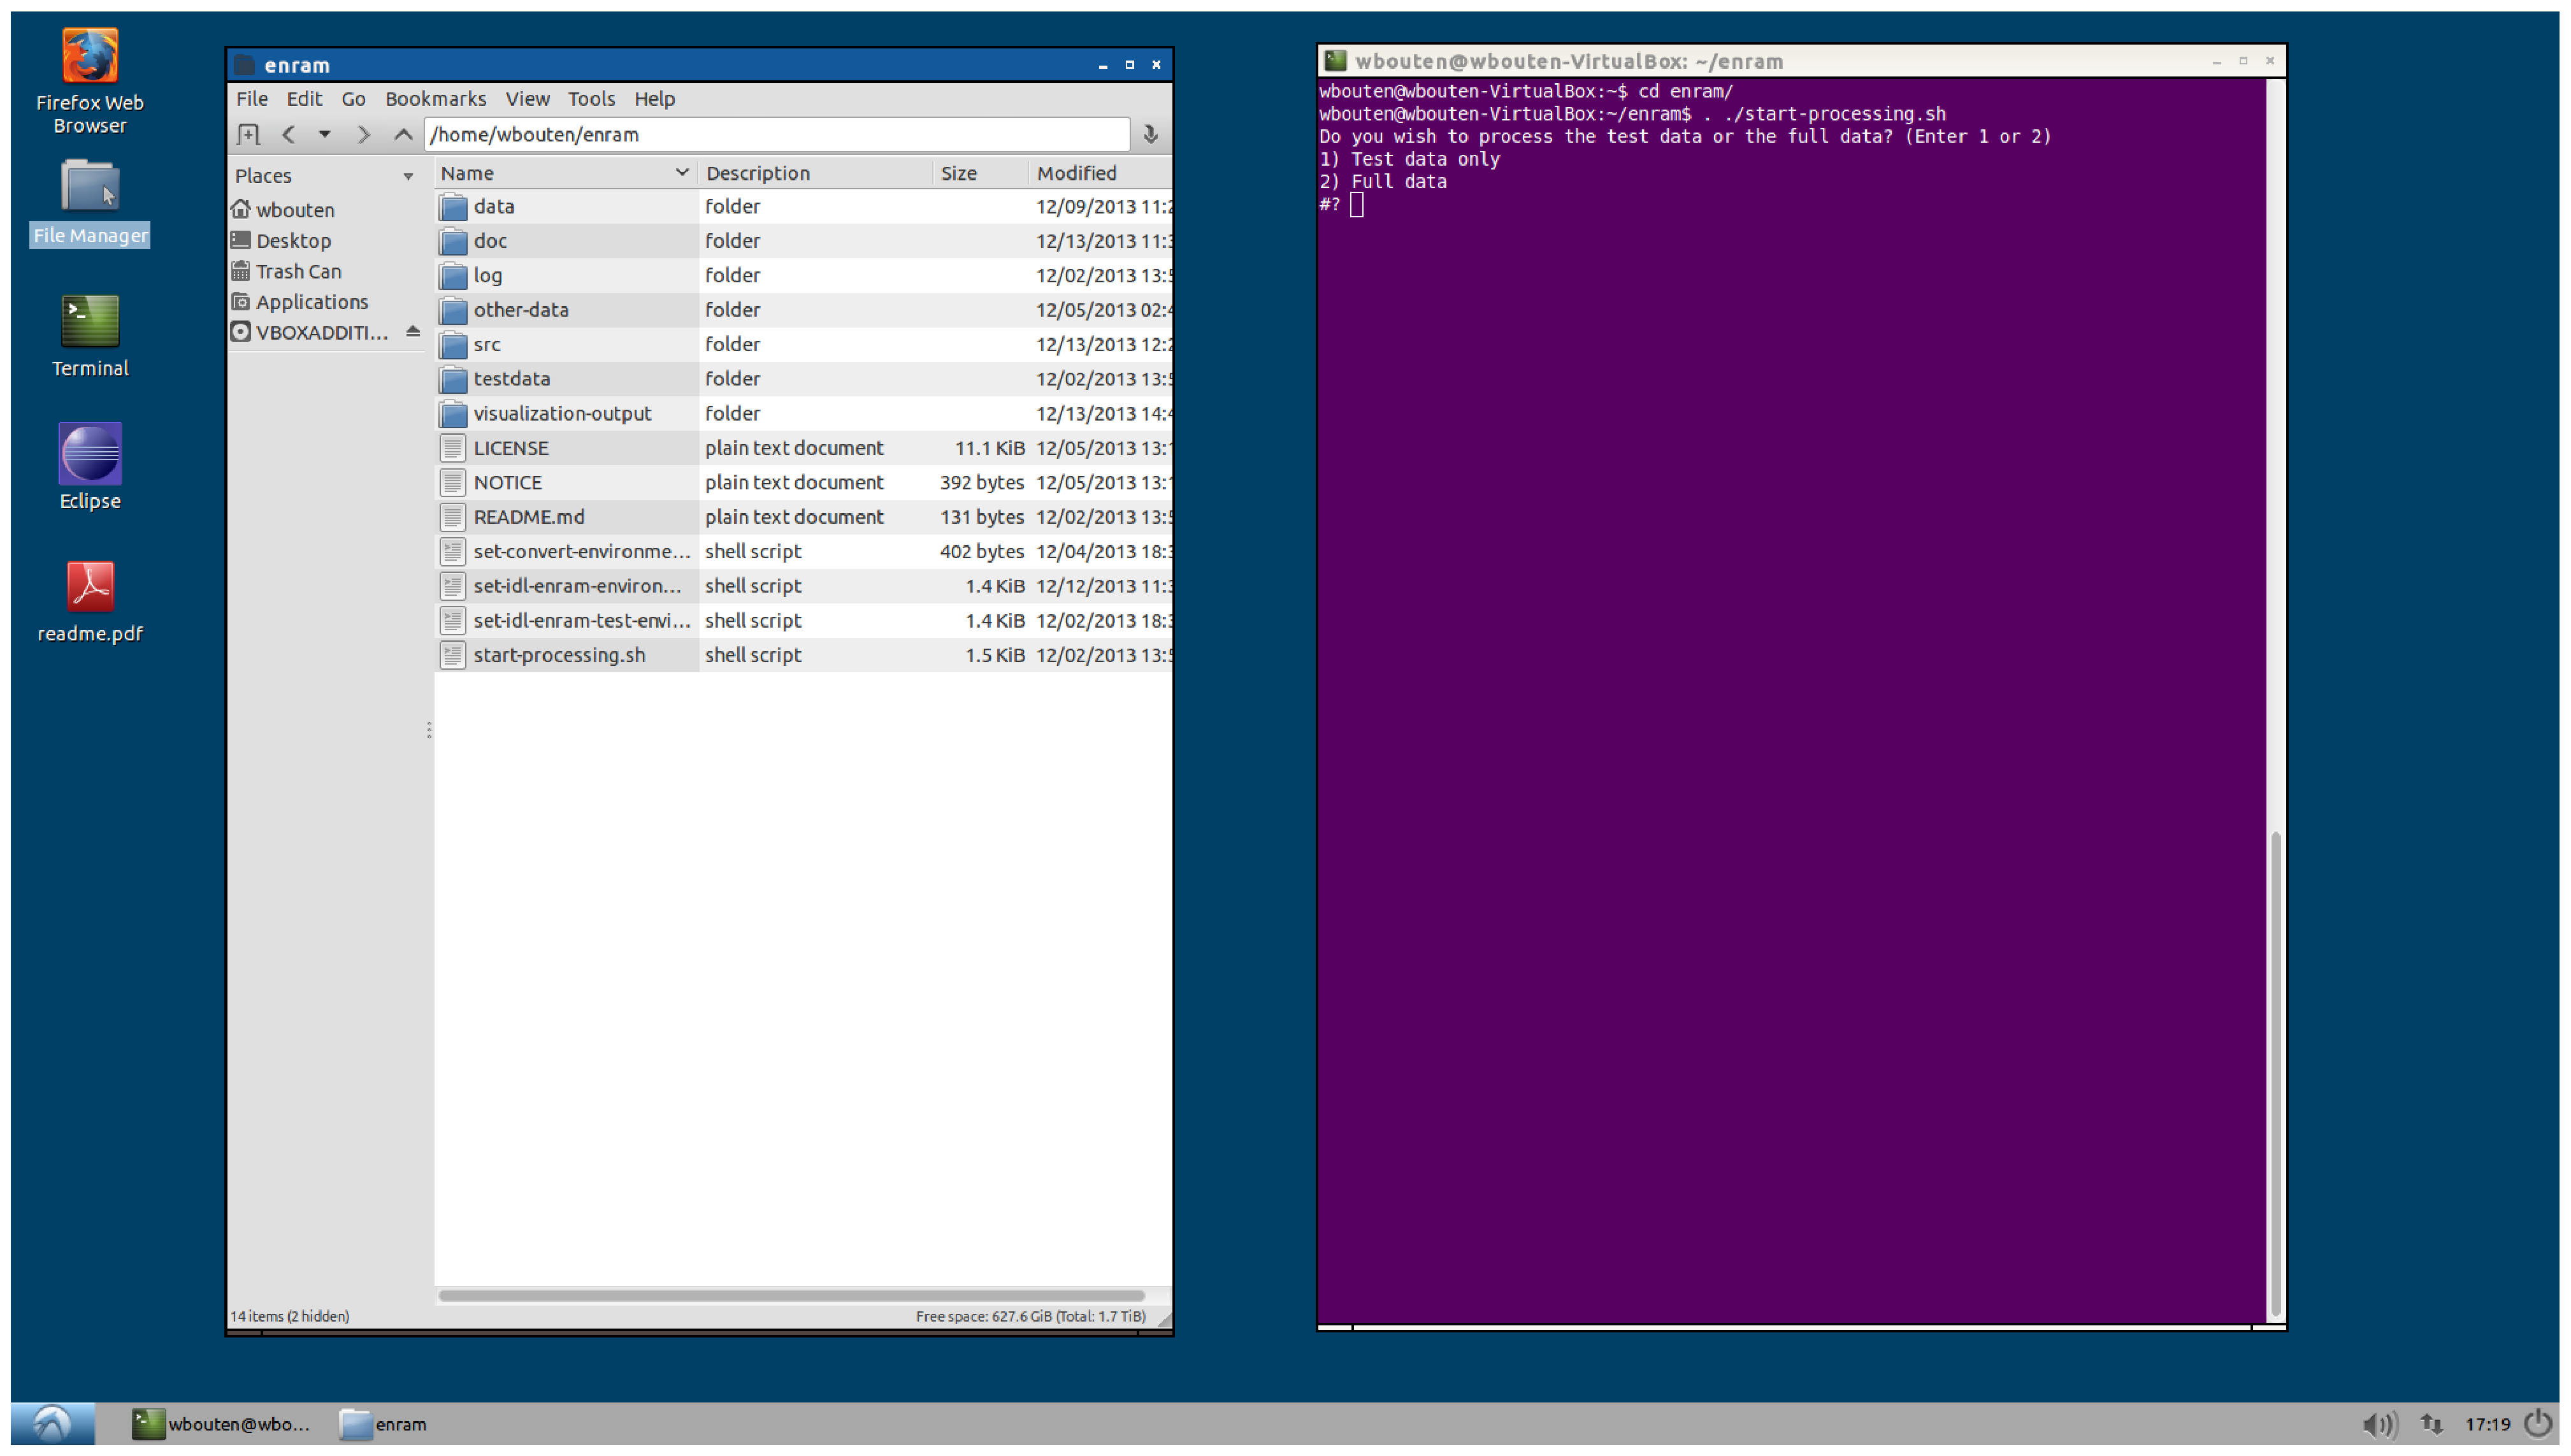
\includegraphics[width=0.85\linewidth , keepaspectratio]{./../eps/screenshot-25.eps}
  \caption{}
  \label{fig:screenshot-25}
\end{figure}

Answer `1' or `2' and press Enter at each question. The terminal will now set up the necessary environment variables.

If you chose to process the data in batch mode, you can use the Firefox web browser to view the batch program's feedback (Figure~\ref{fig:screenshot-26}) while the terminal program is running. Just navigate to `file:///home/wbouten/enram/log/stderr.txt' and `file:///home/wbouten/enram/log/stdout.txt'. Note that these locations have been added to the bookmarks, so if you just type `stderr' or `stdout' in Firefox's URL bar, it should suggest the corresponding files automatically.

\begin{figure}[ht]
  \centering
    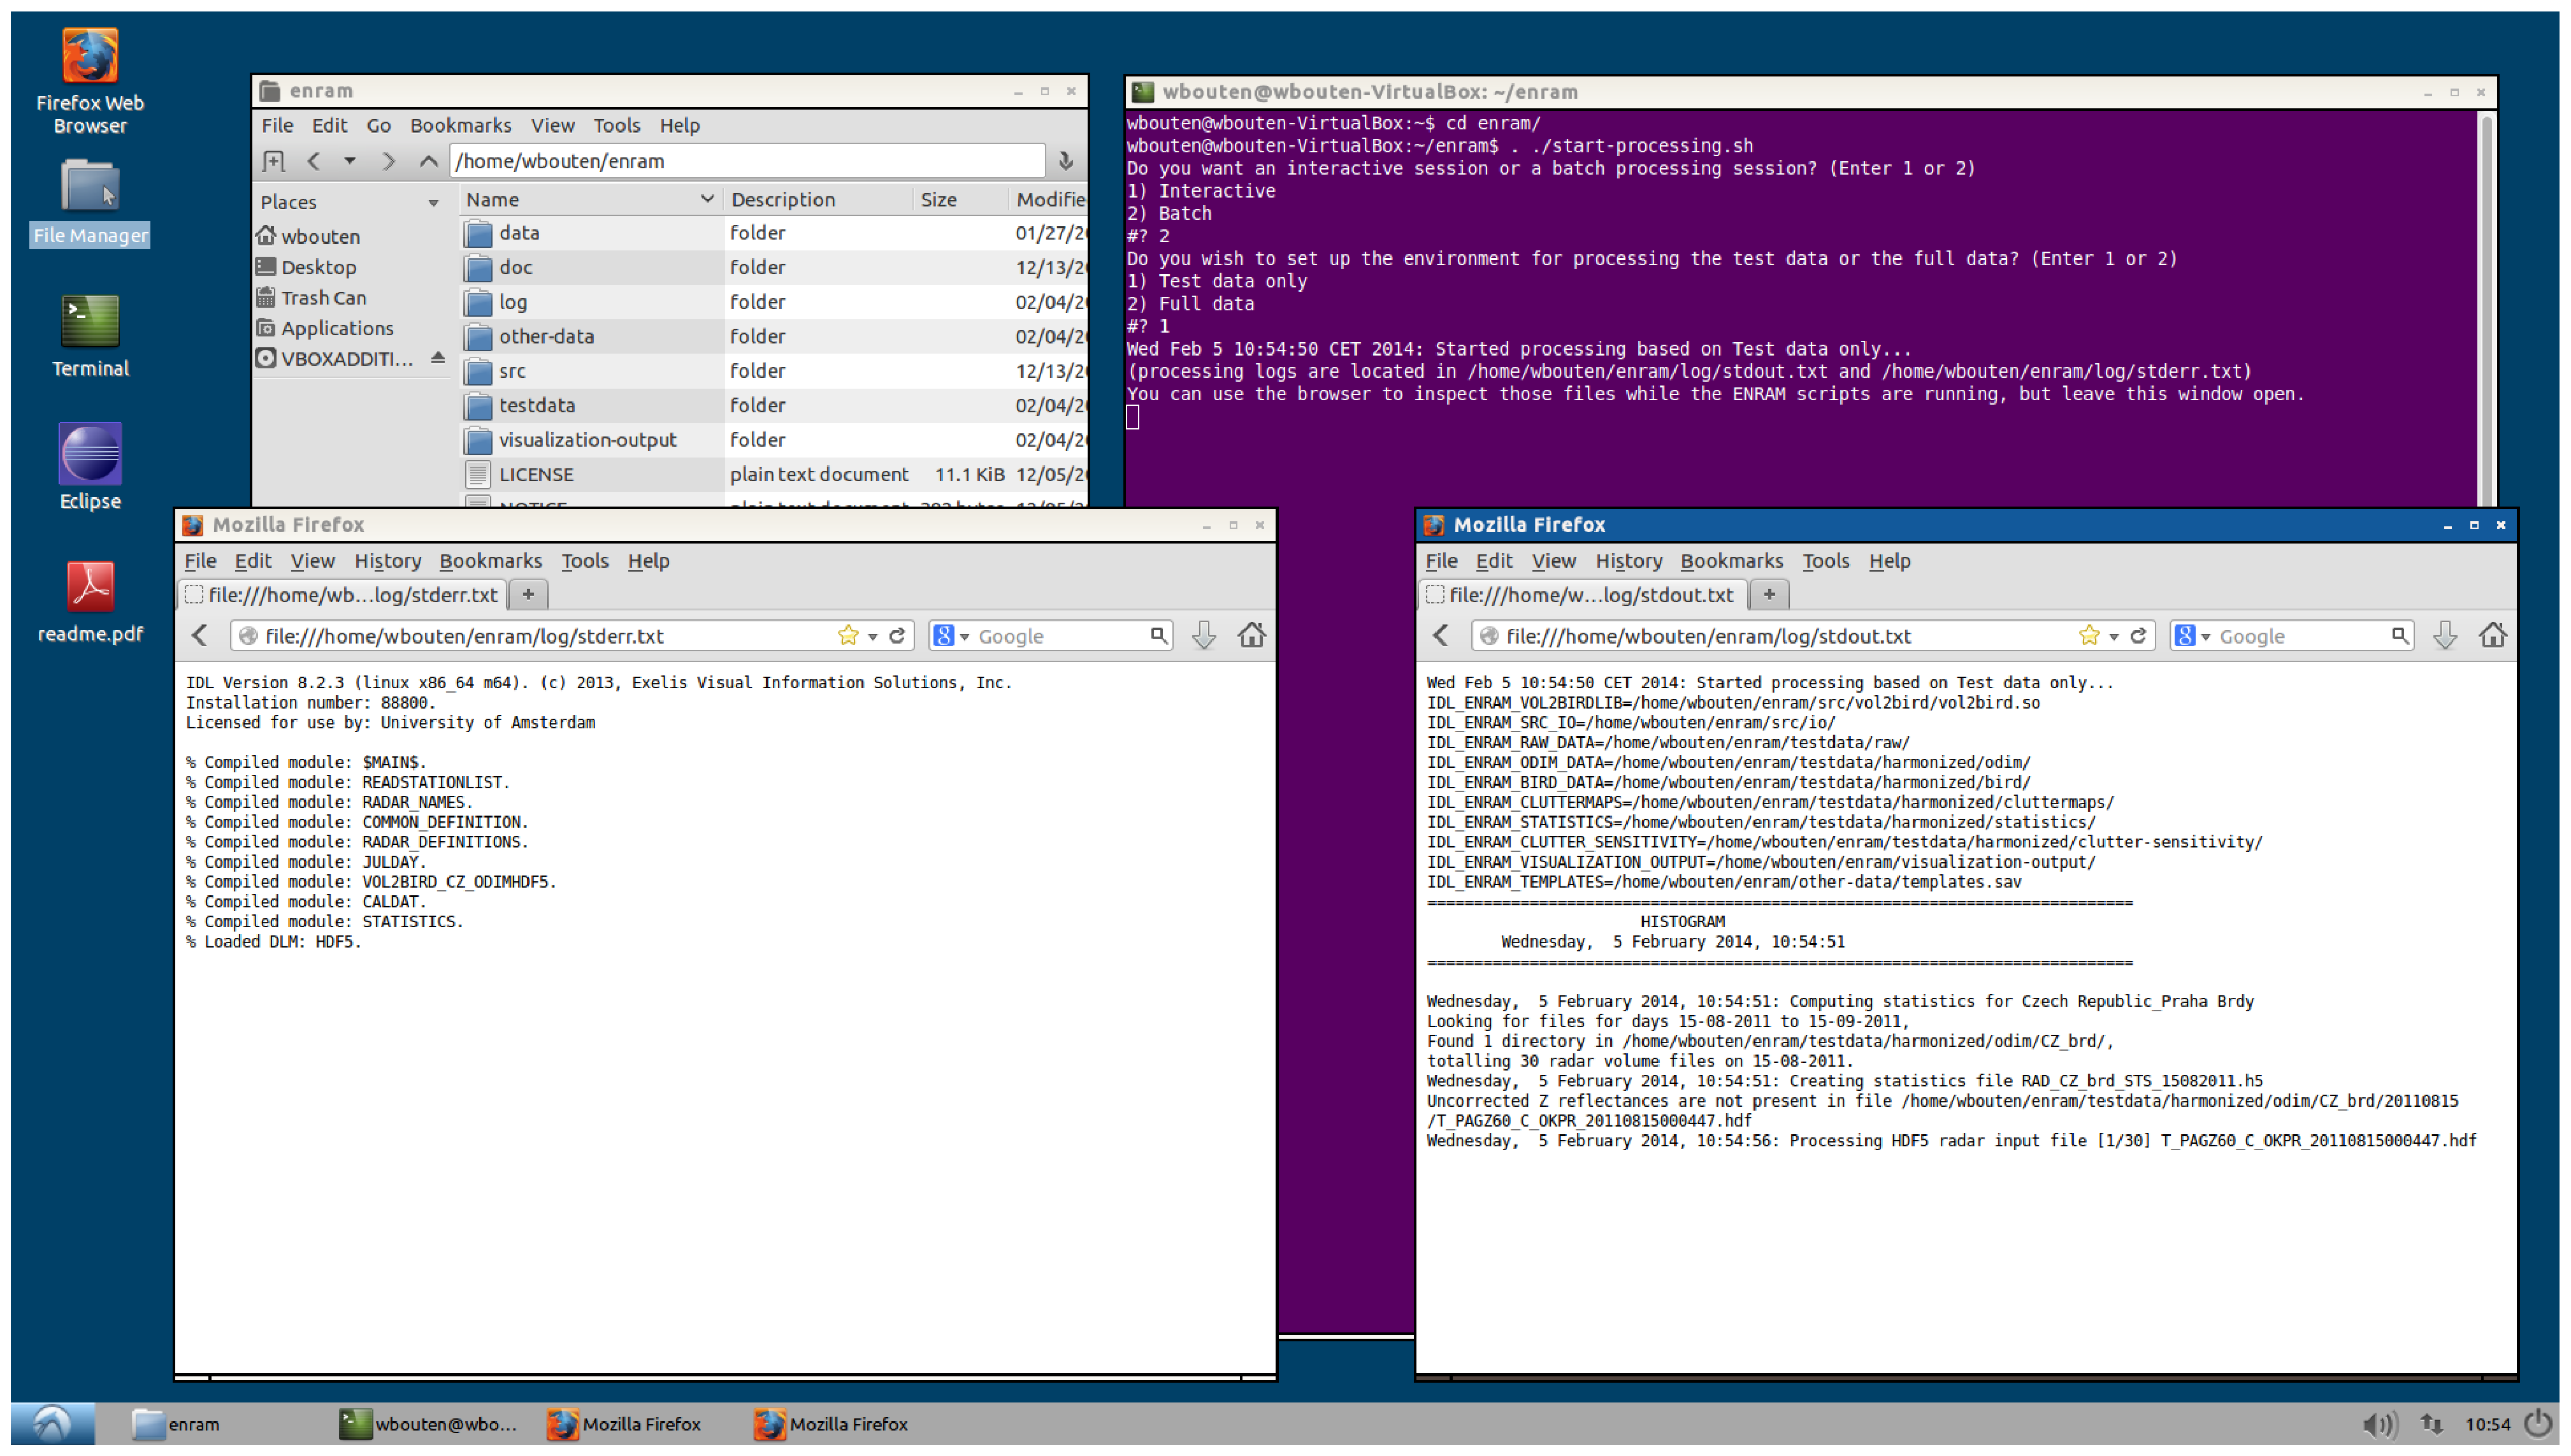
\includegraphics[width=0.85\linewidth , keepaspectratio]{./../eps/screenshot-26.eps}
  \caption{}
  \label{fig:screenshot-26}
\end{figure}

\chapter{Organization of the software}
\label{ch:design-philosophy}


Currently, data from the following stations are included:\\
\\
\begin{longtable}[htb]{ll}
\caption{List of radar stations}
\hline
\textbf{station code} & \textbf{full name}\\
\hline
\endhead
CZBRD & Brdy-Praha, Czech Republic\\
CZSKA & Skalky, Czech Republic \\
FIANJ & Anjalankoski, Finland \\
FIIKA & Ikaalinen, Finland \\
FIKOR & Korpo, Finland \\
FIKUO & Kuopio, Finland \\
FILUO & Luosto, Finland \\
FIUTA & Utaj\"{a}rvi, Finland \\
FIVAN & Vantaa, Finland \\
FIVIM & Vimpeli, Finland \\
FRABB & Abbeville, France \\
FRALE & Al\'{e}ria, France \\
FRAVE & LAvesnois, France \\
FRBLA & Blaisy-Haut, France \\
FRBOL & Boll\`{e}ne, France \\
FRBOR & Bordeaux, France \\
FRBOU & Bourges, France \\
FRCAE & Falaise, France \\
FRCHE & Cherves, France \\
FRCOL & Collobri\`{e}res, France \\
FRGRE & Gr\`{e}zes, France \\
FRMCL & Montclar, France \\
FRMOM & Momuy, France \\
FRMTC & Montancy, France \\
FRNAN & Nancy, France \\
FRNIM & N\^{i}mes, France \\
FRTRO & Arcis-sur-Aube, France \\
HRBIL & Bilogora, Croatia \\
IEDUB & Dublin, Ireland  \\
IESHA & Shannon, Ireland  \\
NLDBL & De Bilt, The Netherlands     \\
NLDHL & Den Helder, The Netherlands \\
NOAND & Andoya, Norway \\
NOBML & Boemlo, Norway \\
NOHAS & Hasvik, Norway \\
NOHGB & Haegebostad, Norway \\
NOHUR & Hurum, Norway \\
NORSA & Rissa, Norway \\
NORST & Rost, Norway \\
NOSTA & Stad, Norway \\
PLBRZ & Brzuchania, Poland \\
PLGDA & Gdansk, Poland \\
PLLEG & Legionowo, Poland \\
PLPAS & Pastewnik, Poland \\
PLPOZ & Pozna\'{n}, Poland \\
PLRAM & Ram\.{z}a, Poland \\
PLRZE & Rzesz\'{o}w, Poland \\
PLSWI & \'{S}widwin, Poland \\
SEANG & \"{A}ngelholm, Sweden \\
SEARL & Stockholm-Arlanda, Sweden \\
SEASE & Ase, Sweden \\
SEHUD & Hudiksvall, Sweden \\
SEKIR & Kiruna, Sweden \\
SEKKR & Karlskrona, Sweden \\
SELEK & Leksand, Sweden \\
SELUL & Lulue\r{a}, Sweden \\
SEOSU & \"{O}stersund, Sweden \\
SEOVI & \"{O}rnsk\"{o}ldsvik, Sweden \\
SEVAR & Vara, Sweden \\
SEVIL & Vilebo, Sweden \\
SILIS & Lisca, Slovenia \\
SKKOH & Kojsovska hola, Slovakia \\
SKMAJ & Maly Javornik, Slovakia\\
\end{longtable}

\needspace{10em}
\section{Directory structure}
The following table lists a selection of the most important files and directories as used in the \mbox{`ENRAMVM'} Virtual Machine.

\begin{longtable}[htb]{lp{7cm}}
\hline
\textbf{Location} & \textbf{Description}\\
(relative to \texttt{/home/wbouten/enram/}) & \\
\hline
\endhead
\texttt{data/}  & conbtains the radar data and derived products \\
\texttt{data/harmonized/bird/}  & contains radar data as HDF5 files after harmonization from zip, gz.tar, gif, etc. \\
\texttt{data/harmonized/cluttermaps/}  & contains cluttermaps for a given station, at different threshold levels of clutter \\
\texttt{data/harmonized/odim/}  & radar data for all stations for the period 15-Aug-2011 to 16-Sep-2011 in ODIM-HDF5 format. \\
\texttt{data/harmonized/statistics/}  & contains output from \texttt{src/process/statistics.pro} \\
\texttt{data/raw/}  & radar data for most stations for the period 15-Aug-2011 to 16-Sep-2011 as provided by individual weather services \\
\texttt{data/stations.txt}  & configuration file containing a list of stations that are part of the data set to be analyzed \\
\texttt{doc/}  & some relevant literature\\
\texttt{doc/readme/}  & the latex files needed for compiling this document\\
\texttt{log/stderr.txt}  &  standard error log\\
\texttt{log/stderr.txt}  & standard output log\\
\texttt{other-data/}  & miscellaneous data (currently not used)\\
\texttt{src/}  & source code main directory\\
\texttt{src/io}  & country-specific i/o routines written in IDL\\
\texttt{src/lib}  & programs and functions from external libraries, written in IDL\\
\texttt{src/process/bird\_call.pro} & IDL program that reads the radial velocity, reflectivity, and cluttermap. and then calls various procedures from Adriaan's library, ultimately resulting in profiles of bird density around a given station.  \\
\texttt{src/process/cluttermap.pro}\footref{fnlabel}  & IDL program that calculates cluttermaps at various thresholds of the statistics data.  Output is written to \texttt{data/harmonized/cluttermaps/}.  \\
\texttt{src/process/flysafe2.pro}  & IDL program that loops over a range of dates and various clutter threshold levels, and then calls \texttt{bird\_call.pro}. \\
\texttt{src/process/histogram.pro}\footref{fnlabel}  & IDL program that loops over a range of dates and stations, and then calls \texttt{statistics.pro}. \\
\texttt{src/process/statistics.pro}  & IDL program that calculates a histogram that serves as a base for constructing cluttermaps later. Output is written to \texttt{data/harmonized/statistics/} \\
\multicolumn{2}{l}{\texttt{src/raw-to-odim-conversion-tools}}\\
 & (incomplete) collection of conversion scripts, mostly written in Bash and C, with which the initial conversion was performed to convert the data from \texttt{data/raw} to the ODIM-HDF5 format in \texttt{data/harmonized/odim}.\\
\multicolumn{2}{l}{\texttt{src/visualization/make\_bird\_density\_profiles.pro}\footref{fnlabel}}\\
   & IDL program that creates figures of bird density as a function of time and altitude.\\
\multicolumn{2}{l}{\texttt{src/visualization/make\_colored\_donut\_maps.pro}\footref{fnlabel}} \\
 & IDL program that creates a figure in which the bird density around each radar is plotted as a colored  donut.\\
\multicolumn{2}{l}{\texttt{src/visualization/make\_ppi\_time\_space\_bird\_rain.pro}\footref{fnlabel}}  \\
& IDL program that creates a map of distributed PPI's of rain and of bird density, at given time intervals. \\
\multicolumn{2}{l}{\texttt{src/visualization/multi\_ppi.pro}\footnote{\label{fnlabel}This program is part of the main data processing pipeline, as defined in the Bash script \texttt{start-processing.sh}.}} \\
   & IDL program that visualizes multiple PPI's.\\
\texttt{src/visualization}  & figure-generating programs\\
\texttt{src/vol2bird} & stores Adriaan Dokter's C language program \\
\texttt{testdata/} & subset of \texttt{data/}, used in integration testing\\
\texttt{visualization-output/}  & directory where all visualization programs place their output figure files\\
\end{longtable}



%\clearpage
%\addappheadtotoc
%\appendixpage
%\begin{appendices}
%%
%\end{appendices}

\backmatter

%\bibliographystyle{plainnat}
%\bibliography{./../bib/literaturedb}


%\printindex
\insertemptypage{}

\end{document}
